%-*- coding: UTF-8 -*-
% notes.tex
%
\documentclass[UTF8]{article}
\usepackage{geometry}
\geometry{a4paper, centering, scale=0.8}
\usepackage{minted}
\usepackage{hyperref}
\usepackage{indentfirst}    % to indent the first paragraph of a section
\usepackage{graphicx}       % to insert figures
\usepackage{amsmath}        % to type some math equations
\usepackage{amssymb}        % to use some special math font
\usepackage{IEEEtrantools}  % to use IEEEeqnarray
\usepackage{algorithm2e}    % to use algorithm environment
\usepackage{mathtools}      % to use \lfloor etc.
\usepackage{multicol}       % to display some content in multi-columns
\setlength{\columnseprule}{0.4pt}   % set the rule's width of multicols
\setlength{\columnsep}{5em}         % set the sep of multicols

% Math notation
% refered to https://github.com/exacity/deeplearningbook-chinese/blob/master/math_symbol.tex
\newcommand{\Scalar}[1]{\mathit{#1}}                % Scalar, the default math font
\newcommand{\Vector}[1]{\boldsymbol{\mathit{#1}}}   % Vector
\newcommand{\Matrix}[1]{\boldsymbol{\mathit{#1}}}   % Matrix
\newcommand{\Tensor}[1]{\textsf{\textbf{#1}}}       % Tensor
\newcommand{\Set}[1]{\mathbb{#1}}                   % Set
\newcommand{\Cal}[1]{\mathcal{#1}}                  % Math Cal

% Draw the lines in a matrix, which is composed by a series of vectors
\newcommand{\vRule}{\rule{0.3pt}{10mm}}             % vertical rule
\newcommand{\hRule}{\,\rule[1mm]{10mm}{0.3pt}\,}    % horizontal rule

% Ceil and floor
\DeclarePairedDelimiter\ceil{\lceil}{\rceil}
\DeclarePairedDelimiter\floor{\lfloor}{\rfloor}

\title{Deep Learning Specialization \\
        Convolutional Neural Networks}
\author{Du Ang \\ \texttt{du2ang233@gmail.com} }
\date{\today}

\begin{document}
\maketitle

\tableofcontents
\newpage

\section{Foundations of Convolutional Neural Networks}
\subsection{Convolutional Neural Networks}
\subsubsection{Computer Vision}
\paragraph{Computer Vision problems}
\begin{itemize}
    \item Image Classfiication
    \item Object Detection
    \item Neural Style Transfer
\end{itemize}

One of the challenges of Computer Vision problems is that the input can be really big. We want to
use large images to train our model, and if we use a fully-connected network, the huge input
features and so many parameters are not feasible to train.

\subsubsection{Edge Detection Example}
\paragraph{Vertical edge detection}
The convolution operation in programming languages:
\begin{itemize}
    \item Python: \mintinline{python}{conv_forward}
    \item TensorFlow: \mintinline{python}{tf.nn.conv2d}
\end{itemize}

\begin{figure}[htb]
    \centering
    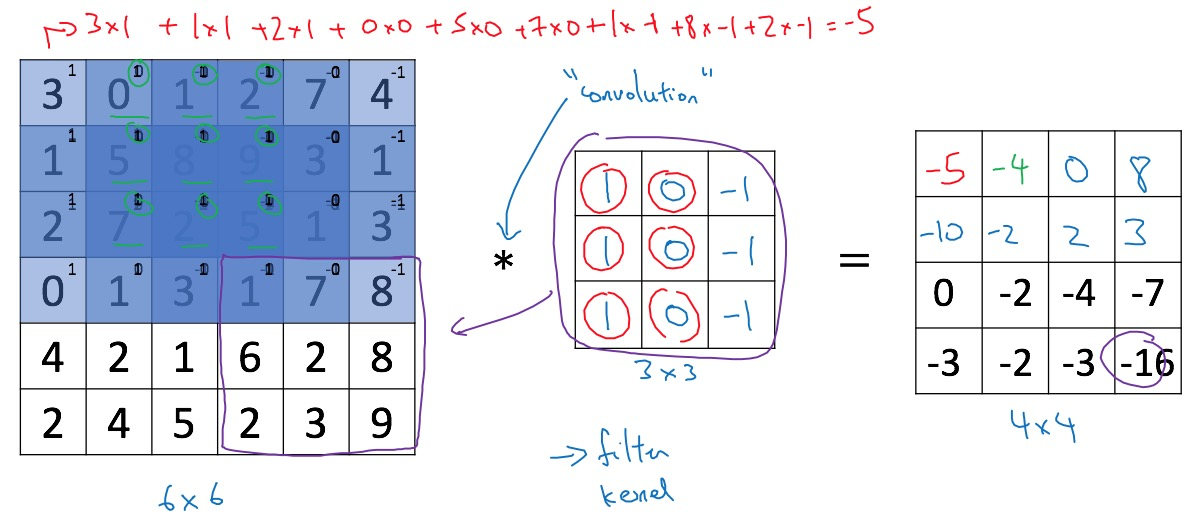
\includegraphics[width=40em]{figures/convolution-operation}
    \caption{The convolution operation for vertical edge detection}
    \label{fig:convolution-operation}
\end{figure}

\begin{figure}[htb]
    \centering
    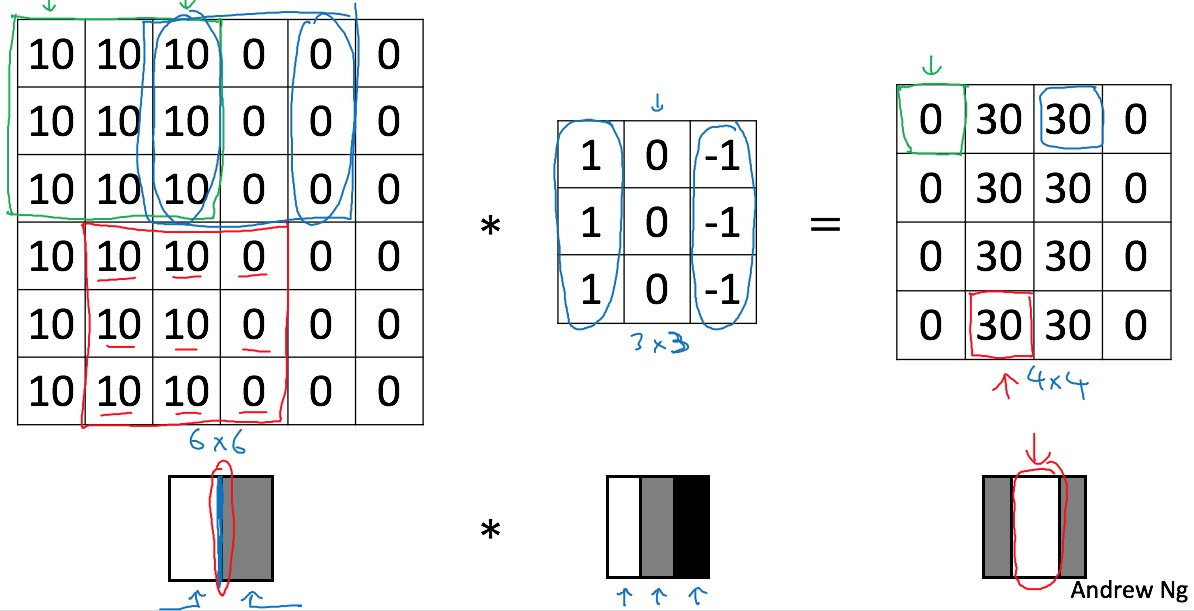
\includegraphics[width=40em]{figures/vertical-edge-detection-example}
    \caption{Vertical edge detection example for a simplified image}
    \label{fig:vertical-edge-detection-example}
\end{figure}

\subsubsection{More Edge Detection}
\begin{figure}[htb]
    \centering
    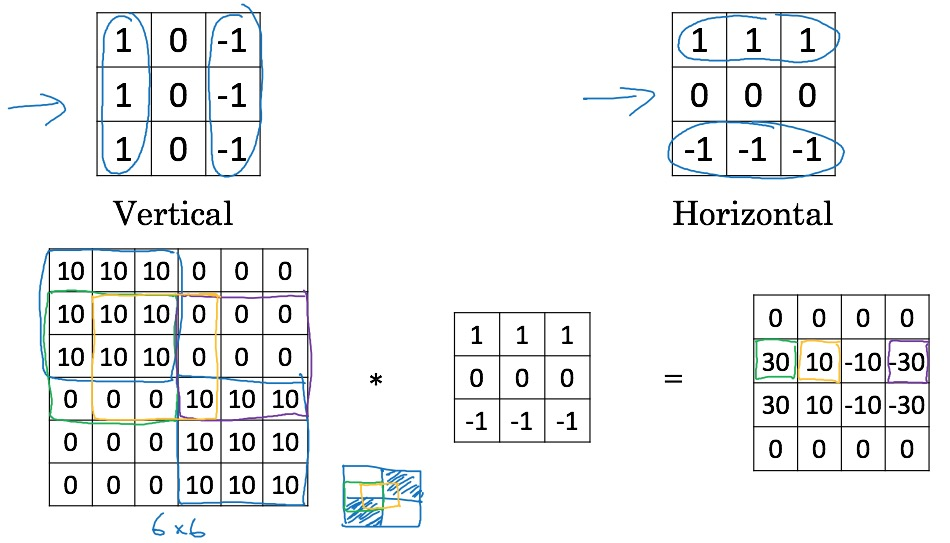
\includegraphics[width=40em]{figures/vertical-and-horizontal-edge-detection-example}
    \caption{Vertical and horizontal edge detection example}
    \label{fig:vertical-and-horizontal-edge-detection-example}
\end{figure}

\paragraph{Learning to detect edges}
Like Figure~\ref{fig:learning-to-detect-edges} shows, the idea that you can treat the nine numbers
in the filter as parameters, has been one of the most powerful ideas in computer vision.

\begin{figure}[htb]
    \centering
    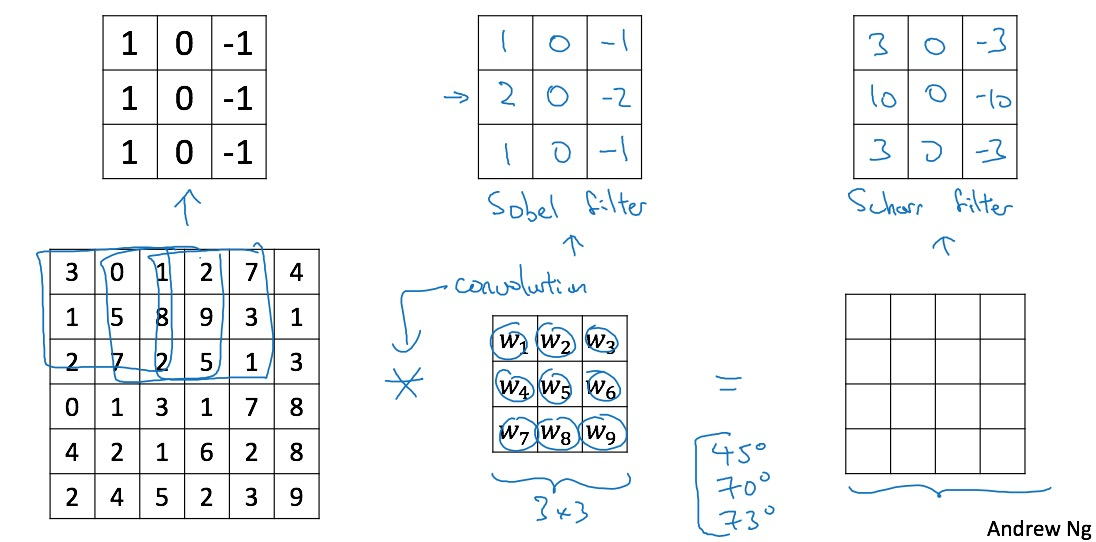
\includegraphics[width=40em]{figures/learning-to-detect-edges}
    \caption{Edge detection example with parameters to learn}
    \label{fig:learning-to-detect-edges}
\end{figure}

\subsubsection{Padding}
For a $n \times n$ image, use a $f \times f$ filter to do convolution, we will get a $(n-f+1) \times
(n-f+1)$ output.

The problems of no padding:
\begin{itemize}
    \item shrinking output
    \item throwing away information from edge
\end{itemize}

\paragraph{Valid and Same convolutions}
\begin{itemize}
    \item ``Valid'': $n \times n \* f \times f \rightarrow (n-f+1) \times (n-f+1)$
    \item ``Same'': Pad so that output size is the same as the input size.
    If we add padding $p$, the output will be $(n+2p-f+1) \times (n+2p-f+1)$, $\displaystyle
    p = \frac{f-1}{2}$. In convention, $f$ is usually odd.
\end{itemize}

\subsubsection{Strided Convolutions}
Strided convolutions is another piece of the basic builiding block of convolutions as used in
convolutional neural networks.

\begin{figure}[htb]
    \centering
    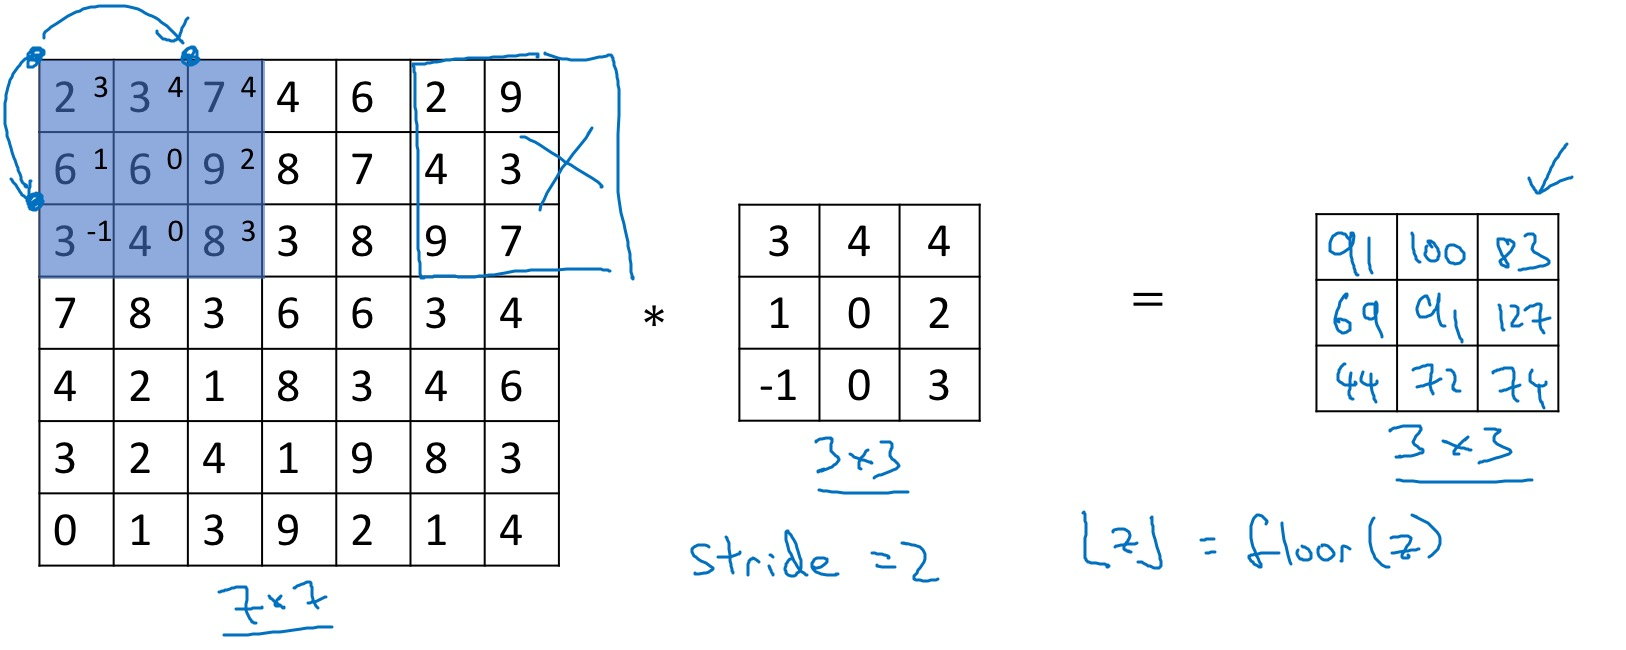
\includegraphics[width=40em]{figures/strided-convolution}
    \caption{Strided convolution example with stride 2}
    \label{fig:strided-convolution}
\end{figure}

$$ n \times n \text{ image (padding } p \text{)} \quad * \quad f \times f \text{ filter (stride }
s \text{)}  \quad \rightarrow \quad \floor*{\frac{n+2p-f}{s}+1} \times \floor*{\frac{n+2p-f}{s}+1}$$

\paragraph{Technical note on cross-correlation vs. convolution}
Convolution in math textbook and sigal processing has an extra mirroring operation, but in Deep
Learning, we've skipped it by convention. Technically, what we're actually doing, is sometimes
called cross-correlation instead of convolution.

The real convolution has the property called associativity in mathematics, which means $(A * B) * C
= A * (B * C)$. This is nice for some signal processing applications, but for deep neural networks,
it really doesn't matter.

\subsubsection{Convolutions Over Volume}
Figure~\ref{fig:convolutions-on-rgb-image} shows the example of convolutions over volume.

\begin{figure}[htb]
    \centering
    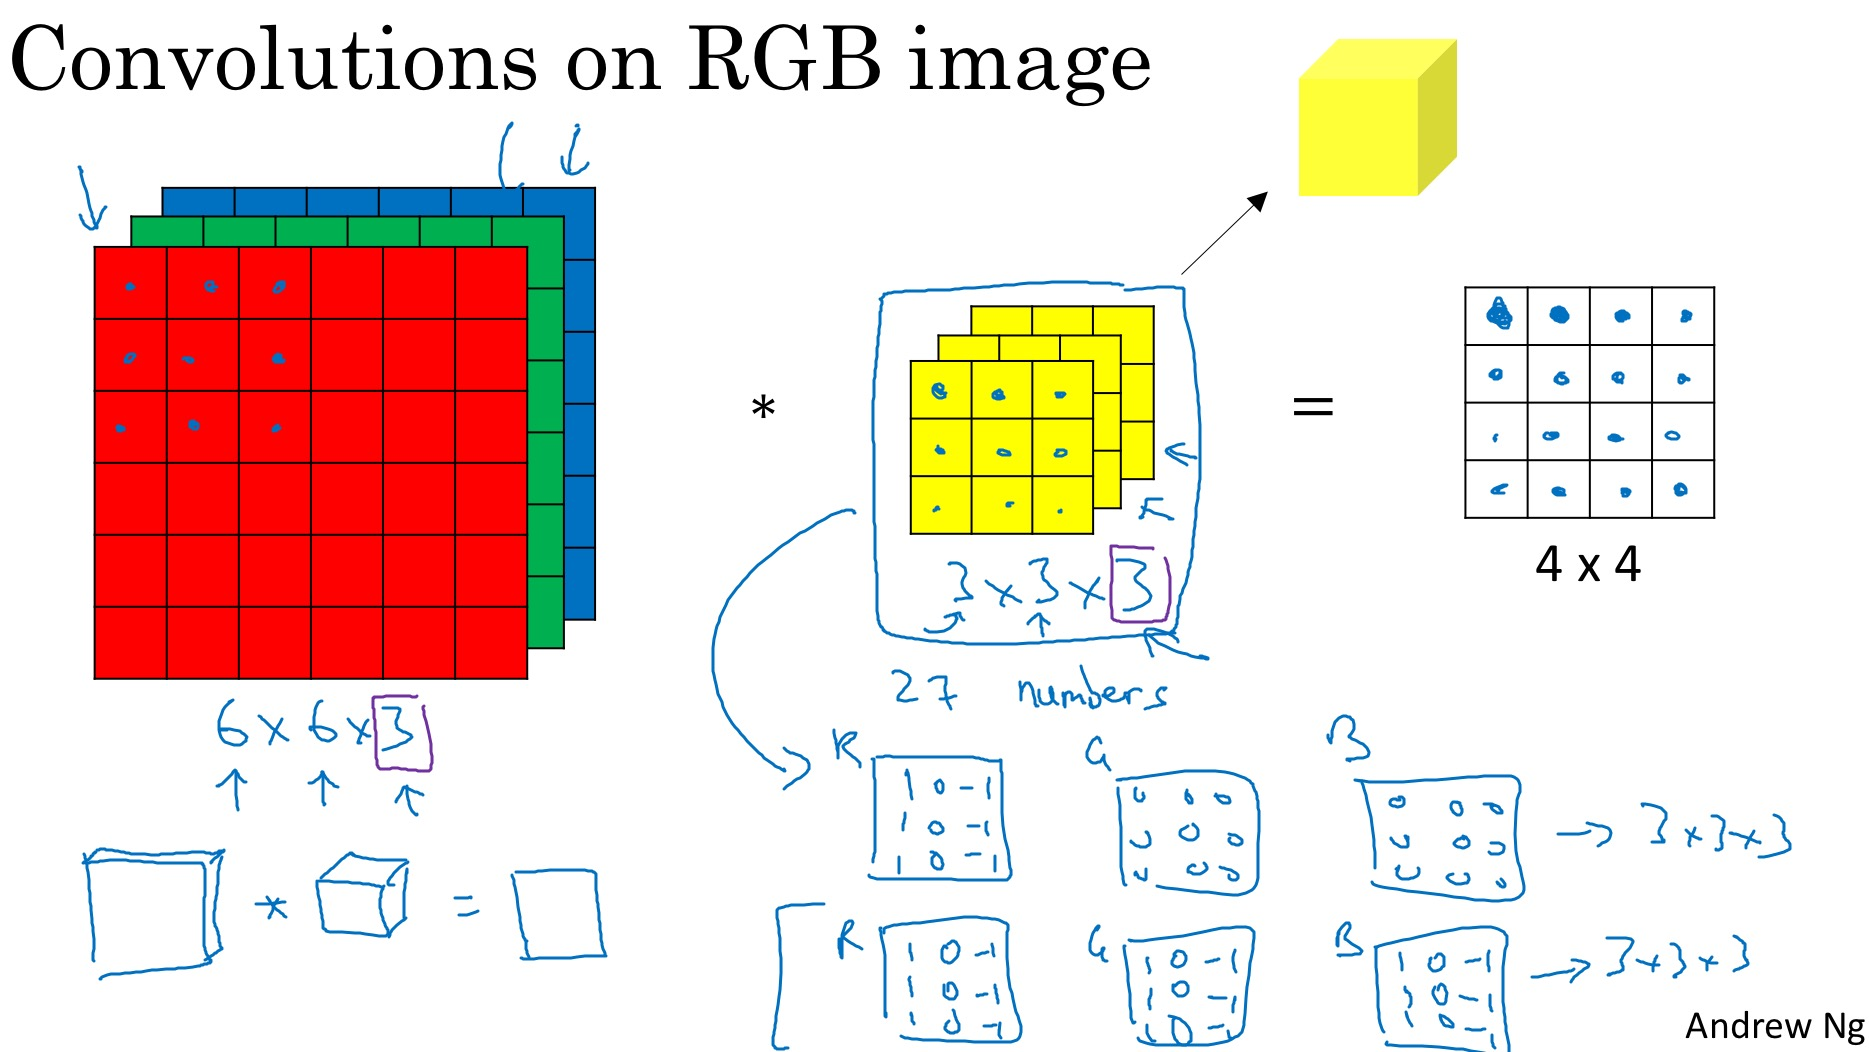
\includegraphics[width=40em]{figures/convolutions-on-rgb-image}
    \caption{Convolutions on RGB image}
    \label{fig:convolutions-on-rgb-image}
\end{figure}

If we want to detect different features at the same time, we can use multiple filters. The output
will then have a number of channels equal to the features you are detecting.

Sometimes, the term ``channel'' is also called ``depth''.

\paragraph{Summary}
$$ n \times n \times n_C \quad * \quad f \times f \times n_C \quad \rightarrow \quad
(n-f+1) \times (n-f+1) \times n_C' \qquad (stride = 1, \text{no padding})$$

\subsubsection{One Layer of a Convolutional Network}
Figure~\ref{fig:example-of-a-conv-layer} shows an example of a layer of a convolutional network.

\begin{figure}[htb]
    \centering
    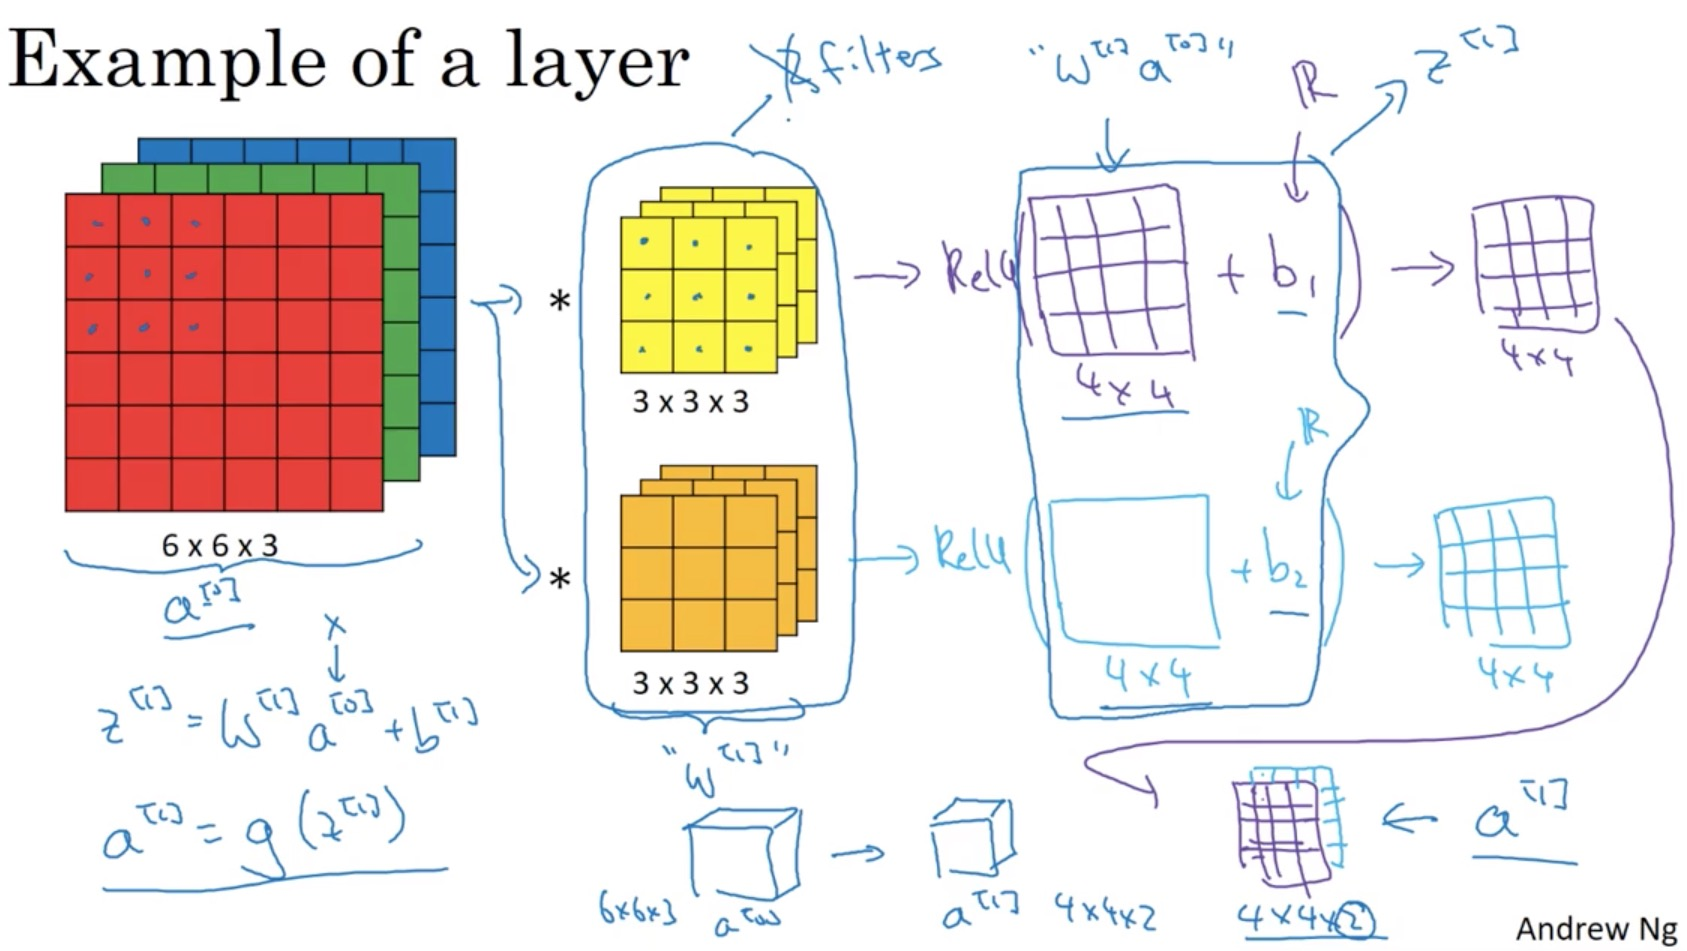
\includegraphics[width=40em]{figures/example-of-a-conv-layer}
    \caption{A example of a convolutional layer}
    \label{fig:example-of-a-conv-layer}
\end{figure}

\paragraph{Number of parameters in one layer}
If you have 10 filters that are $3 \times 3 \times$ in one layer of a neural network, how many
parameters does that layer have?
$$ (3 \times 3 \times 3 + 1) \times 10 = 280 $$

\paragraph{Summary of notation}
If layer $l$ is a convolution layer:
\begin{itemize}
    \item $f^{[l]} = \text{filter size}$
    \item $p^{[l]} = \text{padding}$
    \item $s^{[l]} = \text{stride}$
    \item $n_{\text{C}}^{[l]} = \text{number of filters}$
    \item Each filter is: $f^{[l]} \times f^{[l]} \times n_{\text{C}}^{[l]}$
    \item Activations: $\Vector{a}^{[l]} \rightarrow n_{\text{H}}^{[l]} \times n_{\text{W}}^{[l]} \times
    n_{\text{C}}^{[l]} \qquad \Matrix{A}^{[l]} \rightarrow m \times n_{\text{H}}^{[l]} \times
    n_{\text{W}}^{[l]} \times n_{\text{C}}^{[l]}$
    \item Weights: $f^{[l]} \times f^{[l]} \times n_{\text{C}}^{[l]} \times n_{\text{C}}^{[l-1]}$
    \item bias: $n_{\text{C}}^{[l]} \rightarrow (1, 1, 1, n_{\text{C}}^{[l]})$
    \item Input: $n_{\text{H}}^{[l-1]} \times n_{\text{W}}^{[l-1]} \times n_{\text{C}}^{[l-1]}$
    \item Output: $n_{\text{H}}^{[l]} \times n_{\text{W}}^{[l]} \times n_{\text{C}}^{[l]}$
    \item $\displaystyle n_{\text{H/W}}^{[l]} = \floor{\frac{n_{\text{H/W}}^{[l-1]} + 2p^{[l]}
    - f^{[l]}}{s^{[l]}} + 1}$
\end{itemize}

\subsubsection{Simple Convolutional Network Example}
A simple convolutional network example can be seen in Figure~\ref{fig:example-of-a-conv-layer}.

As you go deeper in the neural network, typically you start up with larger images, the height
and width will stay the same for a while, and gradually trend down as you go deeper in your
networks, whereas the number of channels will generally increase.

\begin{figure}[htb]
    \centering
    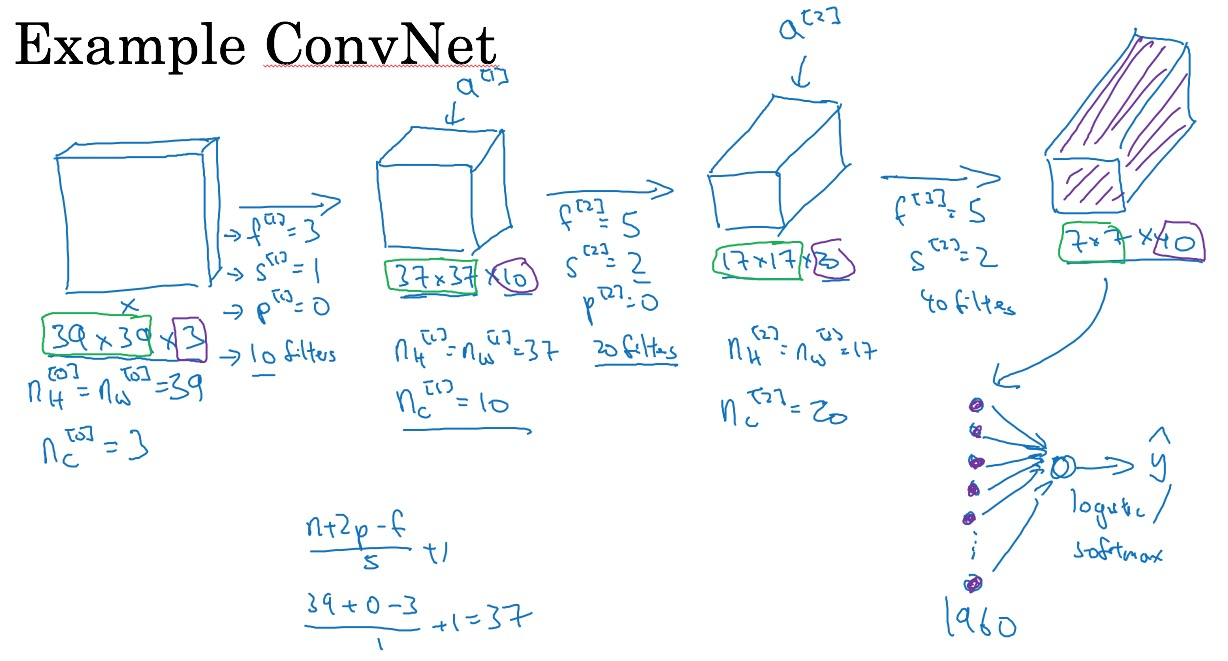
\includegraphics[width=40em]{figures/example-of-a-conv-net}
    \caption{A example of a convolutional network}
    \label{fig:example-of-a-conv-layer}
\end{figure}

Types of layers in a convolutional network:
\begin{itemize}
    \item Convolution (CONV)
    \item Pooling (POOL)
    \item Fully connected (FC)
\end{itemize}

\subsubsection{Pooling Layers}
Figure~\ref{fig:max-pooling} shows what max pooling is. As you can see, each coloured moving window
captures the maximum value within the widow is the output.

\begin{figure}[htb]
    \centering
    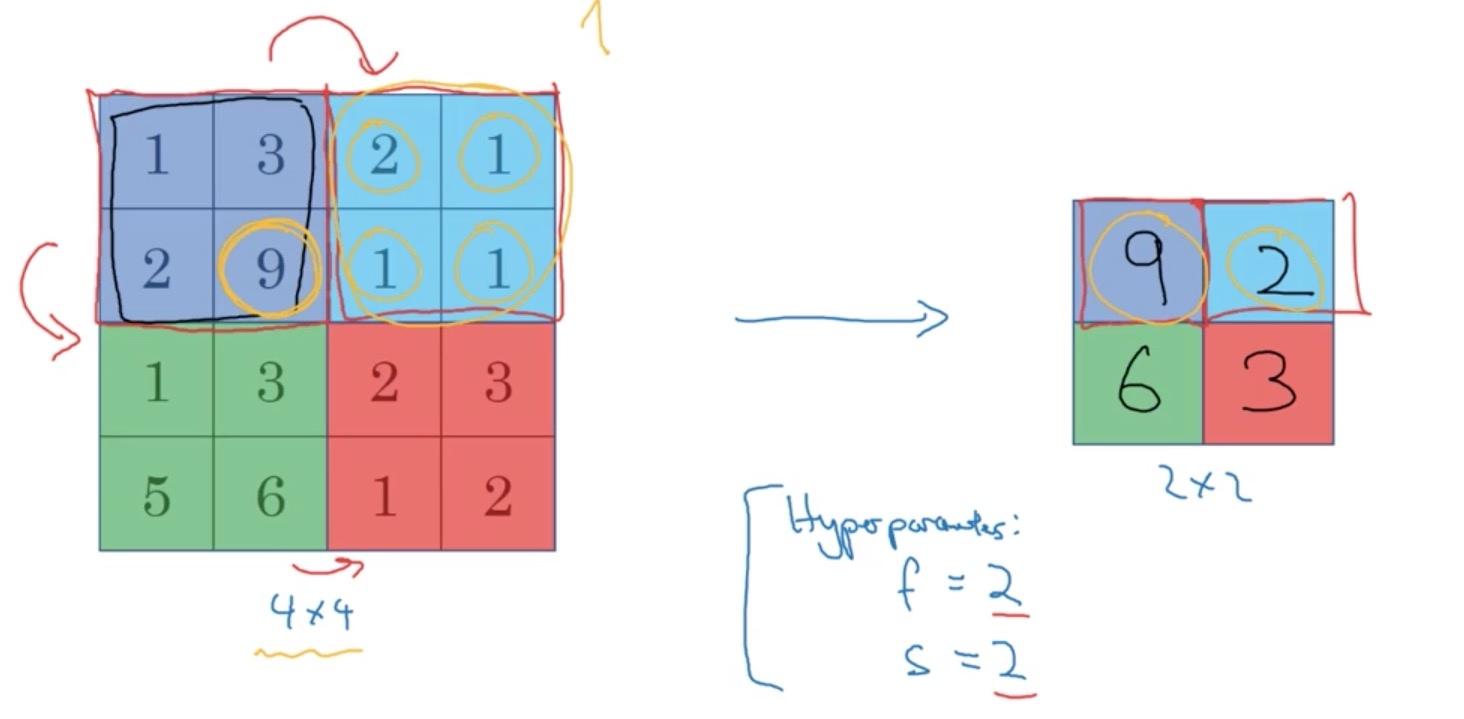
\includegraphics[width=40em]{figures/max-pooling}
    \caption{Max pooling}
    \label{fig:max-pooling}
\end{figure}

Figure~\ref{fig:average-pooling} shows a average pooling example. Instead of taking the maxes
within each filter, you take the average.

\begin{figure}[htb]
    \centering
    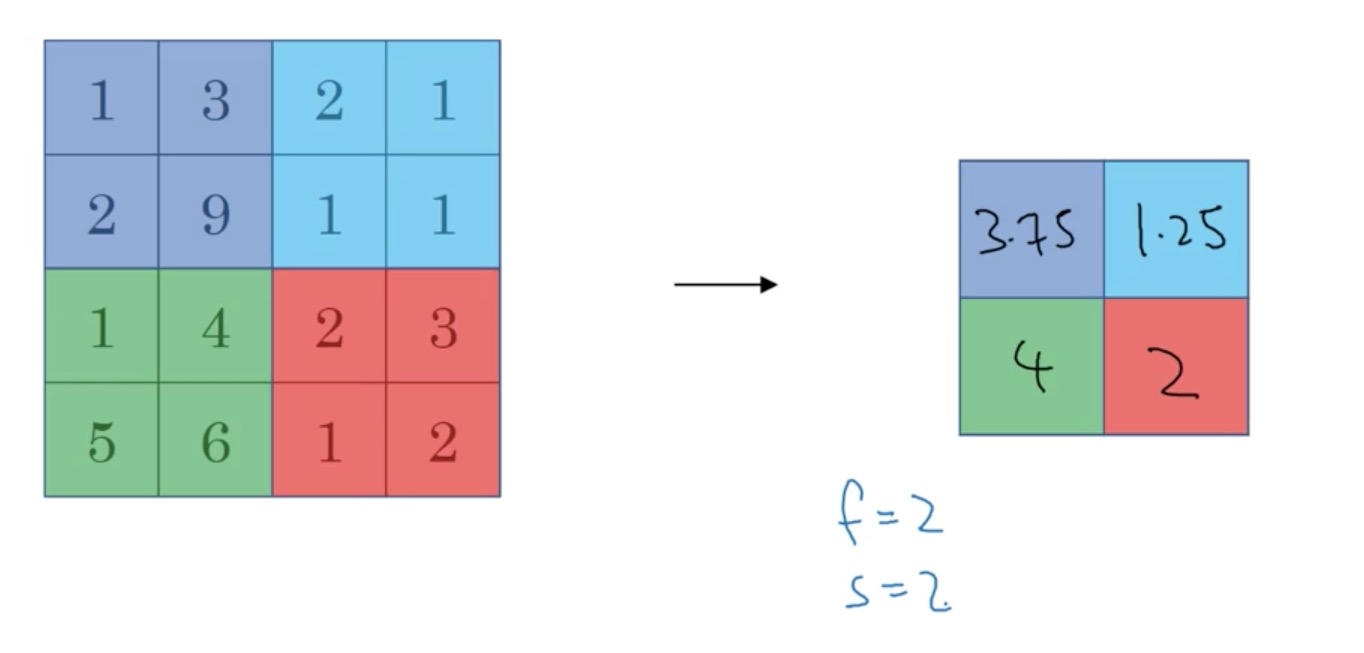
\includegraphics[width=40em]{figures/average-pooling}
    \caption{Average pooling}
    \label{fig:average-pooling}
\end{figure}

These days max pooling is used much more often than average pooling. With one exception, which is
sometimes, very deep in a neural network, you might use average pooling to collapse your
implementation from, say, $7 \times 7 \times 1000$, and average over all to get $1 \times 1 \times
1000$.

Hyperparameters (max or average pooling):
\begin{itemize}
    \item $f$: \text{filter size}
    \item $s$: \text{stride}
    \item ($p$: \text{padding}, little used)
\end{itemize}

Input: $ n_{\text{H}} \times n_{\text{W}} \times n_{\text{C}} $

Output: $\displaystyle \floor*{\frac{n_{\text{H}}-f}{s}+1} \times
\floor*{\frac{n_{\text{W}}-f}{s}+1} \times n_{\text{C}} $

Pooling layers have no parameters to learn.

\subsubsection{CNN Example}
Figure~\ref{fig:cnn-example} shows a CNN example inpired by LeNet-5.

In the literature of a ConvNet, there are two conventions which are slightly in consistence about
what you call a layer. One convention is call CONV+POOL a layer. Another convention would be to
count the CONV layer as a layer, and the POOL layer as a layer. When people report a number of
layers in a neural network, usually people report just the number of layers that have weights
(parameters). In this class, we will use the first convention.

\begin{figure}[htb]
    \centering
    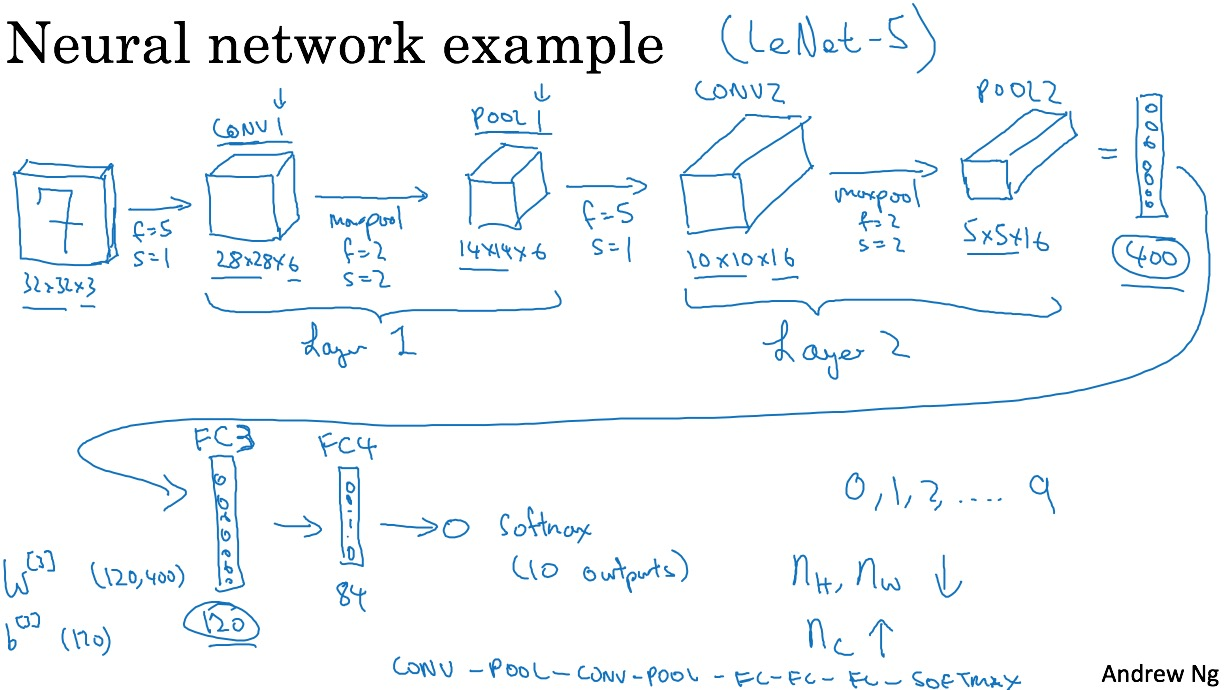
\includegraphics[width=40em]{figures/cnn-example}
    \caption{A CNN example, inspired by LeNet-5}
    \label{fig:cnn-example}
\end{figure}

\begin{figure}[htb]
    \centering
    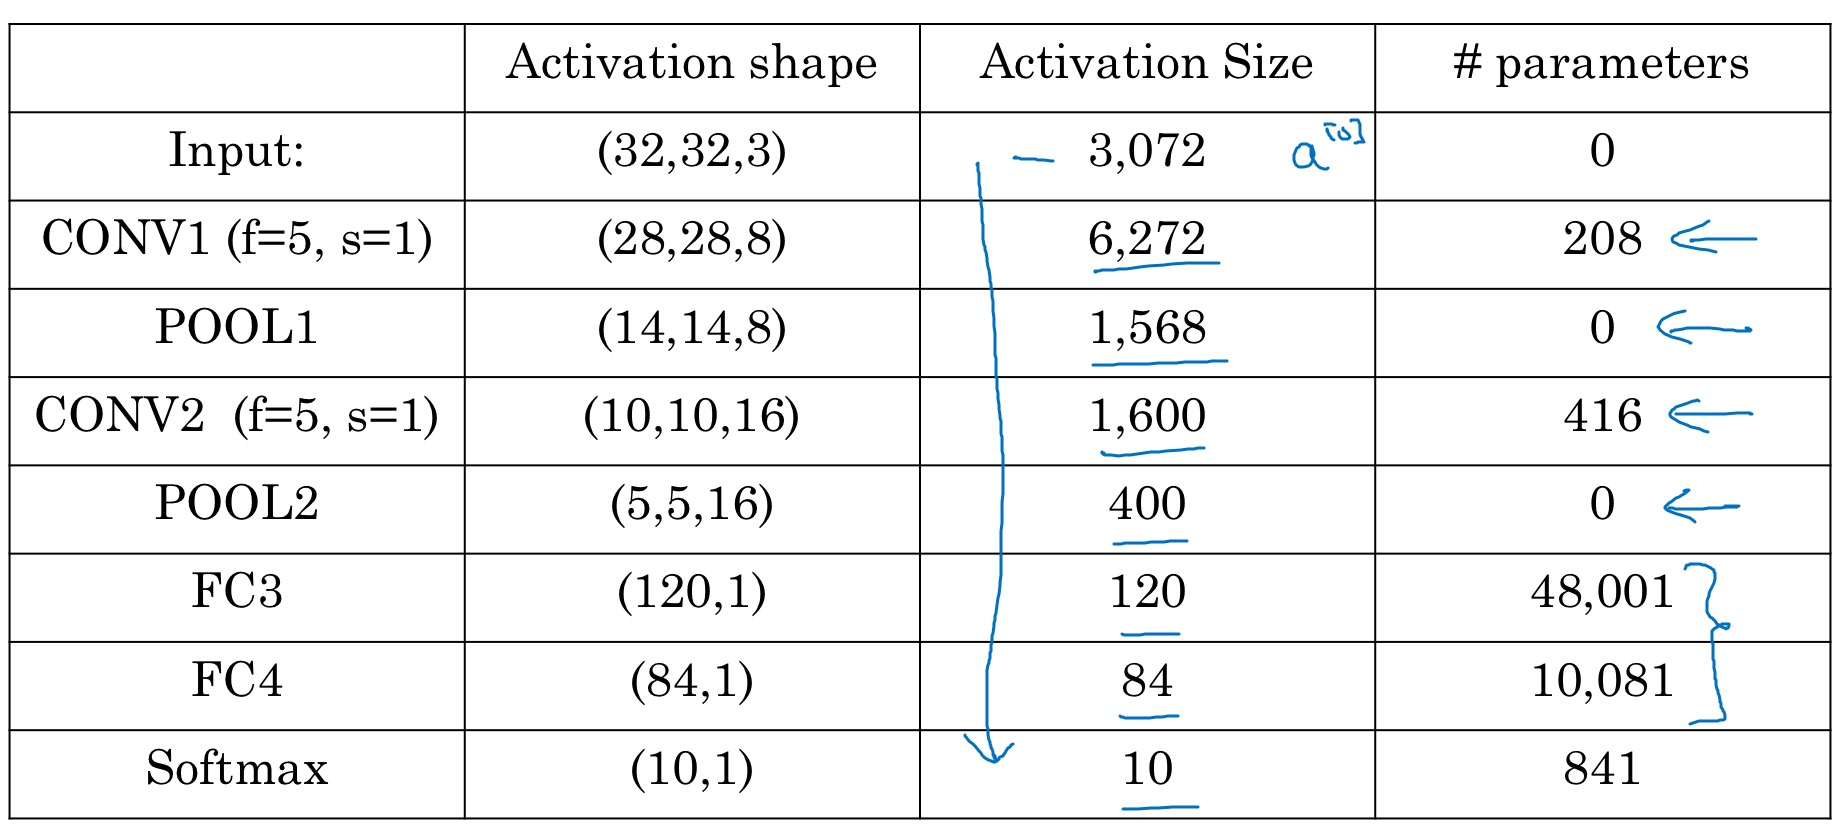
\includegraphics[width=40em]{figures/cnn-example-details}
    \caption{The details of a CNN example, inspired by LeNet-5}
    \label{fig:cnn-example-details}
\end{figure}

\subsubsection{Why Convolutions?}
There are two advantages of convolutional layers over just using fully-connected layers:
\begin{enumerate}
    \item Parameter sharing: A feature detector (such as a vertical edge detector) that's useful in
    one part of the image is probably useful in another part of the image.
    \item Sparsity of connections: In each layer, each output value depends only on a small number
    of inputs.
\end{enumerate}

Convolutional neural networks are very good at capturing translation of the areas, that's because
a convolutional structure helps the neural network encode the fact that an image shifted a few
pixels should result in pretty similar features and should probably be assigned the same output
label.

\section{Deep convolutional models: case studies}
\subsection{Case studies}
\subsubsection{Why look at case studies?}
One of the best ways for you to gain intuition yourself, is to read or to see other examples of
effective components. And it turns out that a neural network architecture that works well on one
computer vision task often works well on other tasks as well.

\paragraph{Outline}
\begin{itemize}
    \item Classic networks
    \begin{itemize}
        \item LeNet-5
        \item AlexNet
        \item VGG
    \end{itemize}
    \item ResNet
    \item Inception
\end{itemize}

\subsubsection{Classic Networks}
LeNet-5 (Figure~\ref{fig:lenet-5}), AlexNet (Figure~\ref{fig:alexnet}), VGG-16
(Figure~\ref{fig:vgg-16})

\begin{figure}[htb]
    \centering
    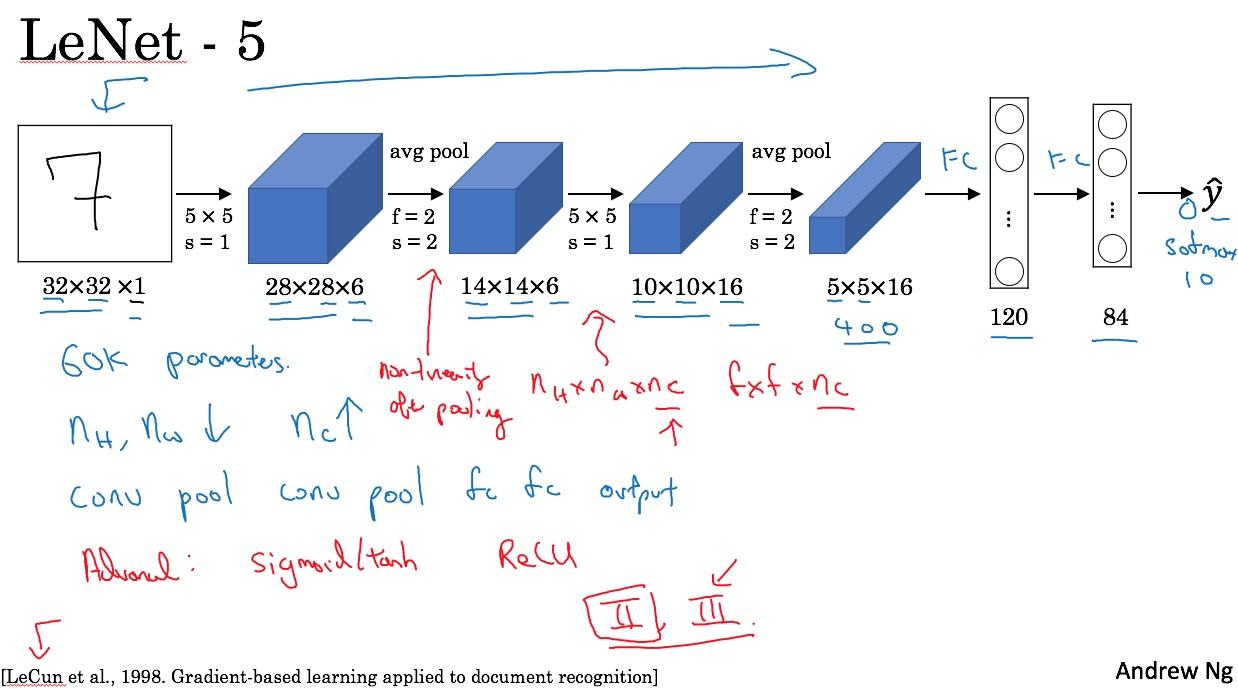
\includegraphics[width=40em]{figures/lenet-5}
    \caption{LeNet-5}
    \label{fig:lenet-5}
\end{figure}

\begin{figure}[htb]
    \centering
    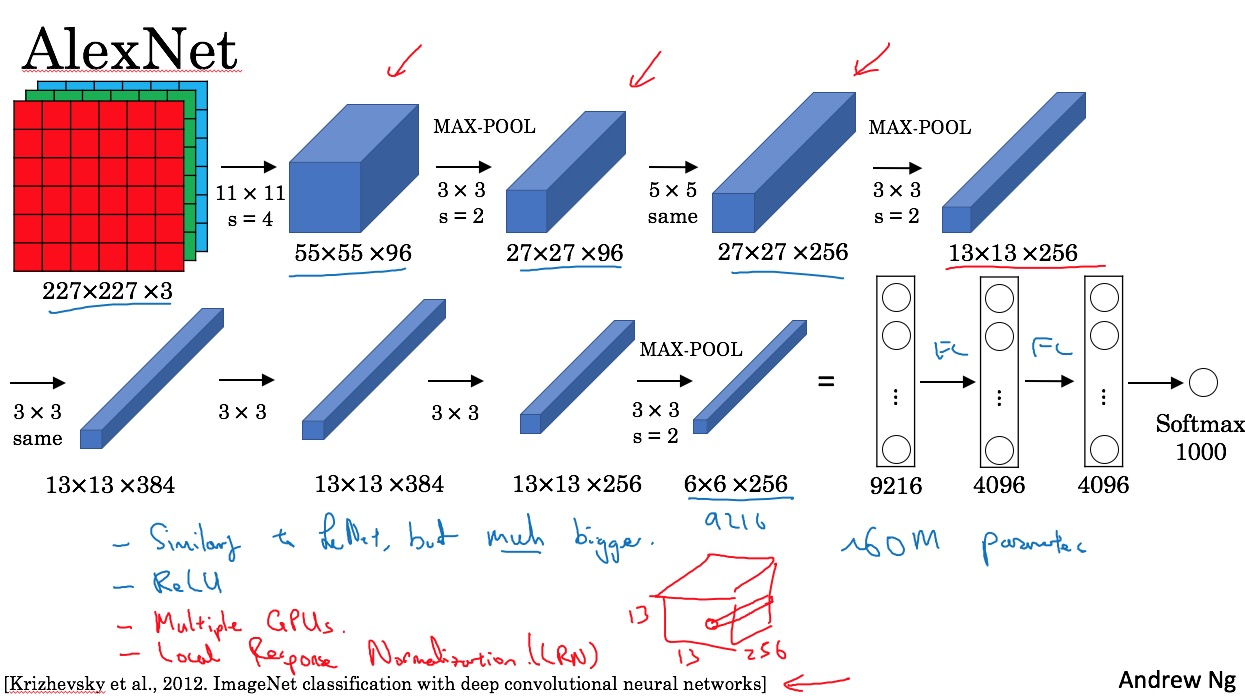
\includegraphics[width=40em]{figures/alexnet}
    \caption{AlexNet}
    \label{fig:alexnet}
\end{figure}

\begin{figure}[htb]
    \centering
    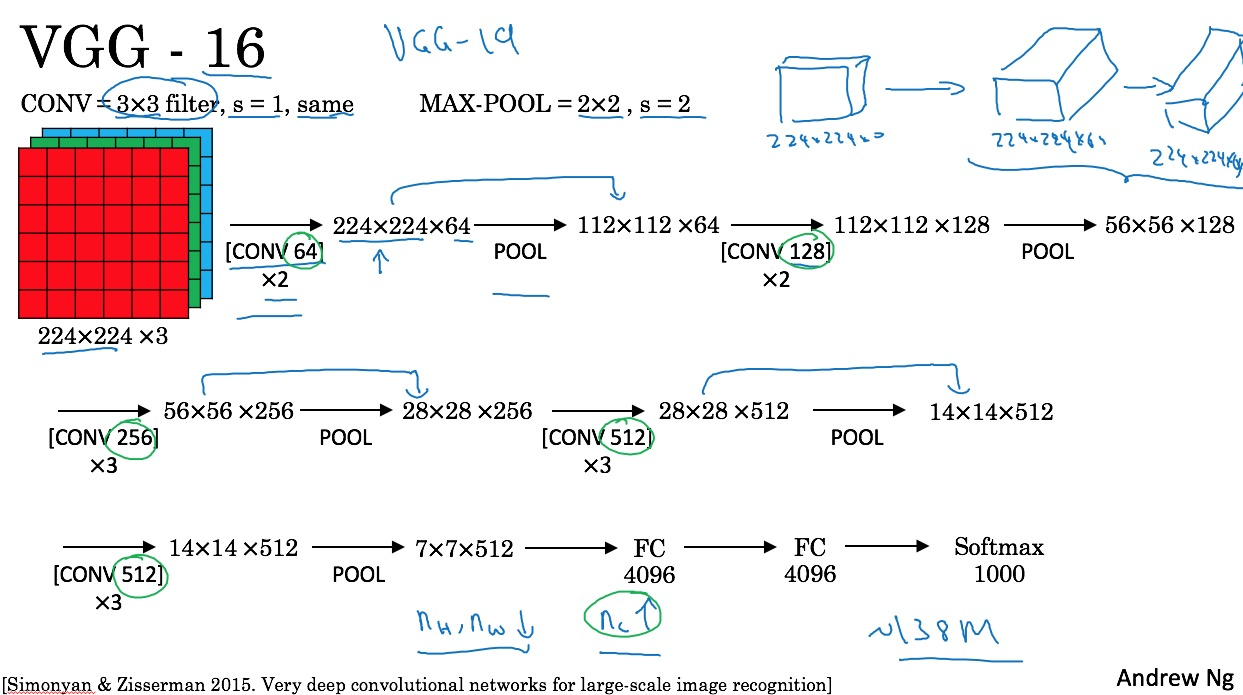
\includegraphics[width=40em]{figures/vgg-16}
    \caption{VGG-16}
    \label{fig:vgg-16}
\end{figure}

\subsubsection{ResNets}
Very, very deep neural networks are difficult to train because of vanishing and exploding gradients
types of problems. Skip connections of ResNets (Figure~\ref{fig:residual-block}) will allow you to
take the activation from one layer and suddenly feed it to another layer, even much deeper in the
neural network.

\begin{figure}[htb]
    \centering
    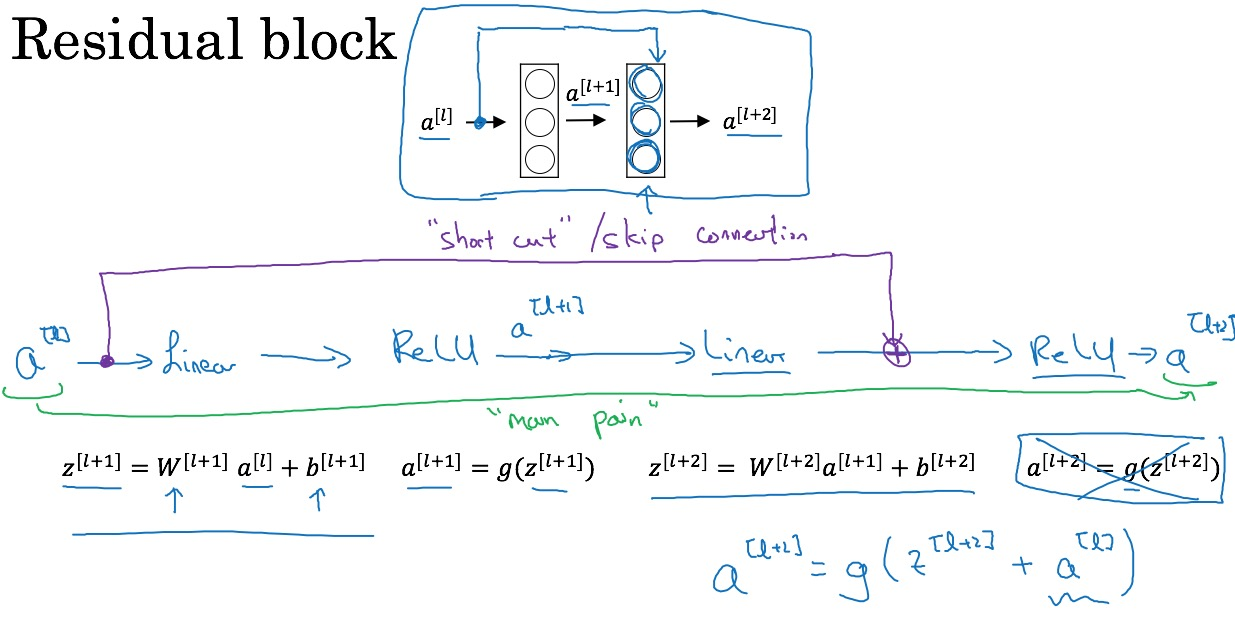
\includegraphics[width=40em]{figures/residual-block}
    \caption{Residual block}
    \label{fig:residual-block}
\end{figure}

$$ \Vector{z}^{[l+1]} = \Matrix{W}^{[l+1]} \Vector{a}^{[l]} + b^{[l+1]} $$
$$ \Vector{a}^{[l+1]} = g(\Vector{z^{[l+1]}}) $$
$$ \Vector{z}^{[l+2]} = \Matrix{W}^{[l+2]} \Vector{a}^{[l+1]} + b^{[l+2]} $$
$$ \Vector{a}^{[l+2]} = g(\Vector{z^{[l+2]}} + \Vector{a}^{[l]}) $$

To turn a ``plain network'' into ResNet, what you do is adding all those skip connections or
shortcut connections.

In theory, as you make a neural network deeper, it should only do better and better on the training
set. But in practice, or in reality, having a plain network that's very deep means that your
optimization algorithm just has a much harder time training, so your training error gets worse if
you pick a network that's too deep. But what happens with ResNets is that even as the number of
layers gets deeper, you can have the performance of the training error kind of keep on going down,
which can be seen in Figure~\ref{fig:plain-res-training-error-compare}.

\begin{figure}[htb]
    \centering
    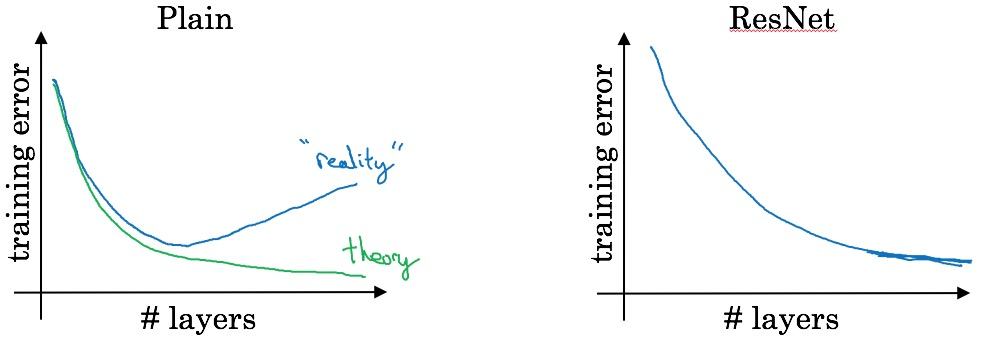
\includegraphics[width=40em]{figures/plain-res-training-error-compare}
    \caption{Comparing of the training error changes between Plain network and ResNet.}
    \label{fig:plain-res-training-error-compare}
\end{figure}

\subsubsection{Why ResNets Work}
$$ \Vector{a}^{[l+2]} = g(\Vector{z^{[l+2]}} + \Vector{a}^{[l]}) $$
$\Vector{z}^{[l+2]} = \Matrix{W}^{[l+2]} \Vector{a}^{[l+1]} + \Vector{b}^{[l+2]}$,
if $\Matrix{W}^{[l+2]} = 0$, $\Vector{b}^{[l+2]} = 0$, then $\Vector{z^{[l+2]}} = 0$
$$ \Vector{a}^{[l+2]} = g(\Vector{a}^{[l]}) = \Vector{a}^{[l]} $$

So Indentity function is easy to for Residual block to learn.

\subsubsection{Networks in Networks and 1 $\times$ 1 Convolutions}
Figure~\ref{fig:network-in-network} shows what is 1 $\times$ 1 convolution and what it does.

\begin{figure}[htb]
    \centering
    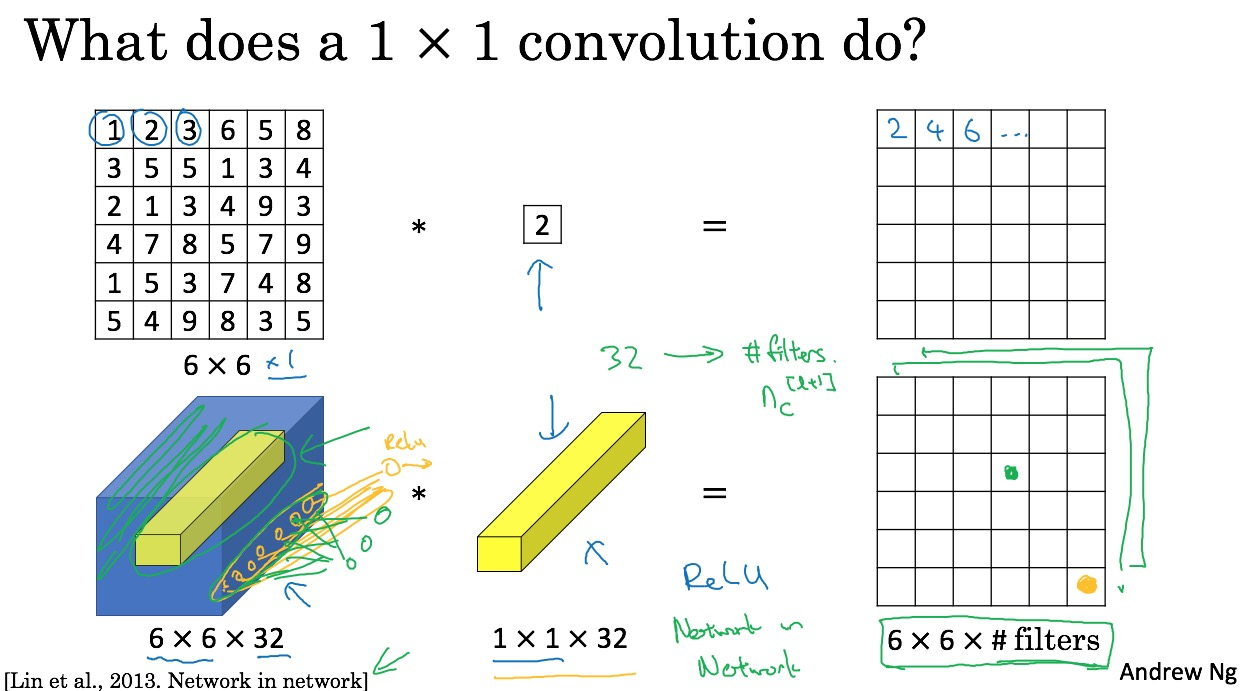
\includegraphics[width=40em]{figures/network-in-network}
    \caption{1 $\times$ 1 convolution (Network in Network)}
    \label{fig:network-in-network}
\end{figure}

Pooling layers can be used to shrink the height and width of a volume, while 1 $\times$
1 convolutions can be used to shink the channels to save on computation.

Just like Figure~\ref{fig:using-1-by-1-conv} shows, if you want to shrink the $28 \times 28 \times
192$ volume to $28 \times 28 \times 32$, you can use 32 $1 \times 1 \times 192$ filters to do 1
$\times$ 1 convolution with it, and you will get a $28 \times 28 \times 32$ output. If you keep the
number of channels at 192, that's fine, and the effect of a 1 $\times$ 1 convolution is it just
adds some nonlinearity, which allows you to learn more complex function of your network.

\begin{figure}[htb]
    \centering
    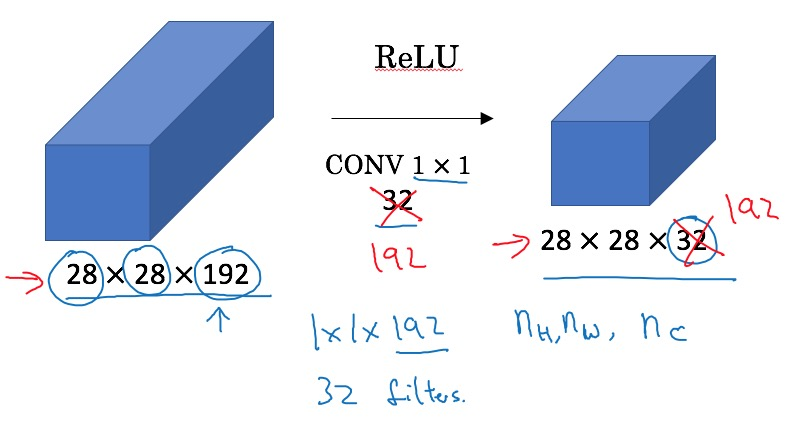
\includegraphics[width=40em]{figures/using-1-by-1-conv}
    \caption{Using 1 $\times$ 1 convolution to shrink the channels of a volume}
    \label{fig:using-1-by-1-conv}
\end{figure}

\subsubsection{Inception Network Motivation}
When designing a layer for a CONV layer, you might have to pick do you want $1 \times 3$ filter,
or $3 \times 3$, or $5 \times 5$. Or do you want to pooling layer? What inception network does is
it says, instead of choosing what filter size you want in a CONV layer or even do you want a
convolutional layer or pooling layer, let's do them all, see Figure~\ref{fig:inception-motivation}.

\begin{figure}[htb]
    \centering
    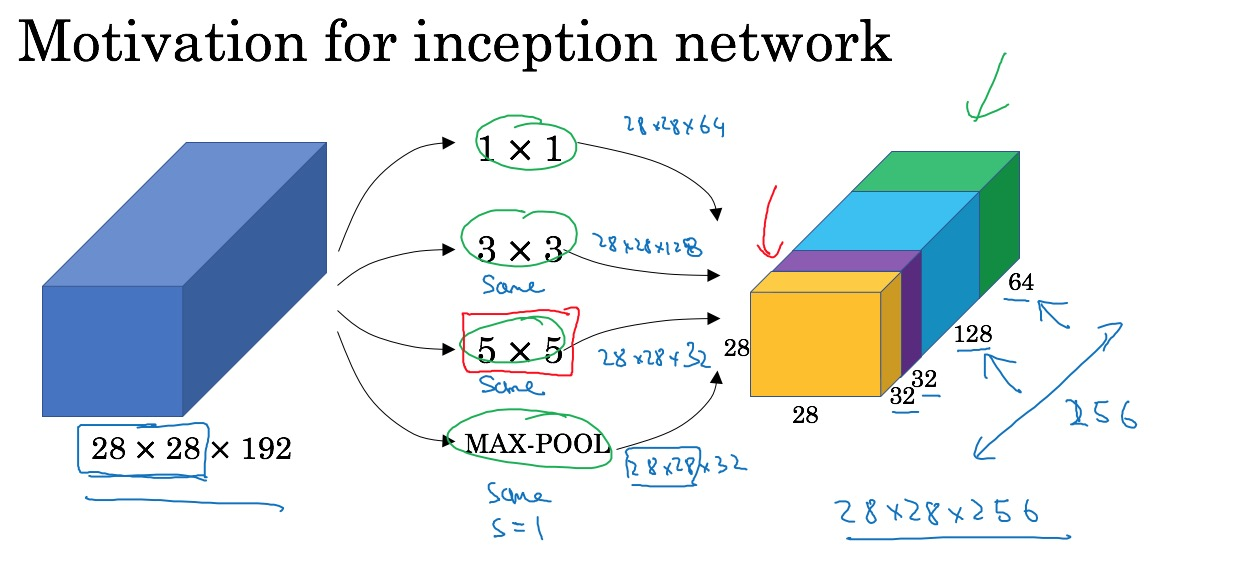
\includegraphics[width=40em]{figures/inception-motivation}
    \caption{The motivation for Inception Network}
    \label{fig:inception-motivation}
\end{figure}

\paragraph{The problem of computational cost}
Like Figure~\ref{fig:using-1-by-1-conv-to-save-computation}, with the help of ``bottleneck layer'',
you can save on computation by using 1 $\times$ 1 convolution.

\begin{figure}[htb]
    \centering
    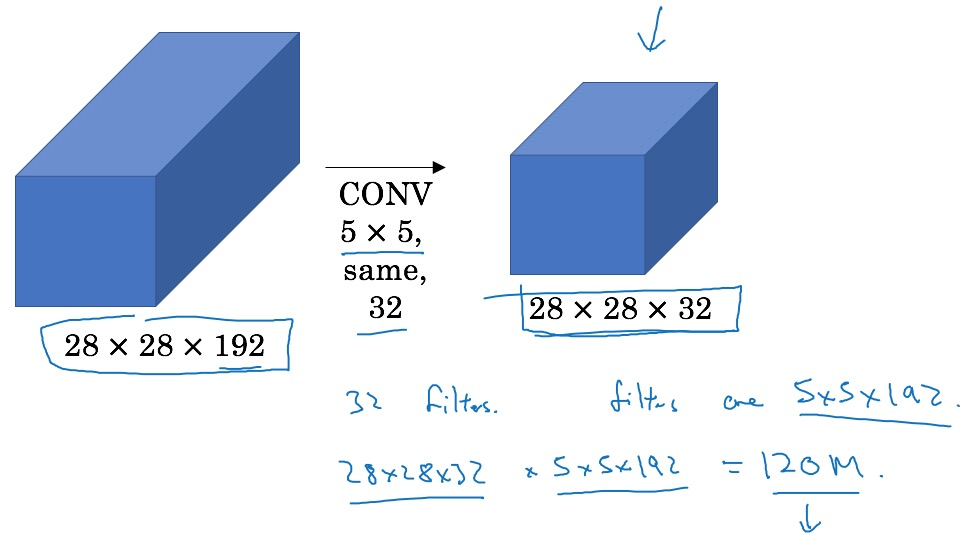
\includegraphics[width=30em]{figures/problem-of-computation-cost}
    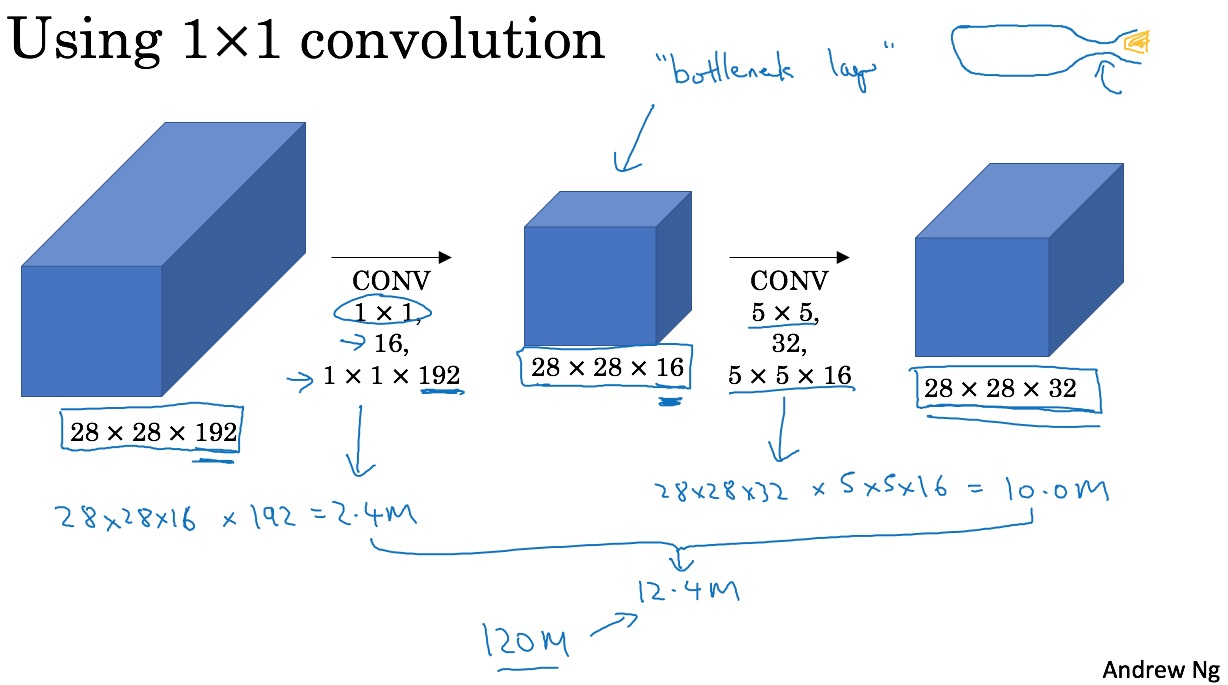
\includegraphics[width=40em]{figures/using-1-by-1-conv-to-save-computation}
    \caption{Using 1 $\times$ 1 convolution to save on computation.}
    \label{fig:using-1-by-1-conv-to-save-computation}
\end{figure}

\subsubsection{Inception Network}
Figure~\ref{fig:inception-module-and-inception-network} shows the Inception module and Inception
Network.

\begin{figure}[htb]
    \centering
    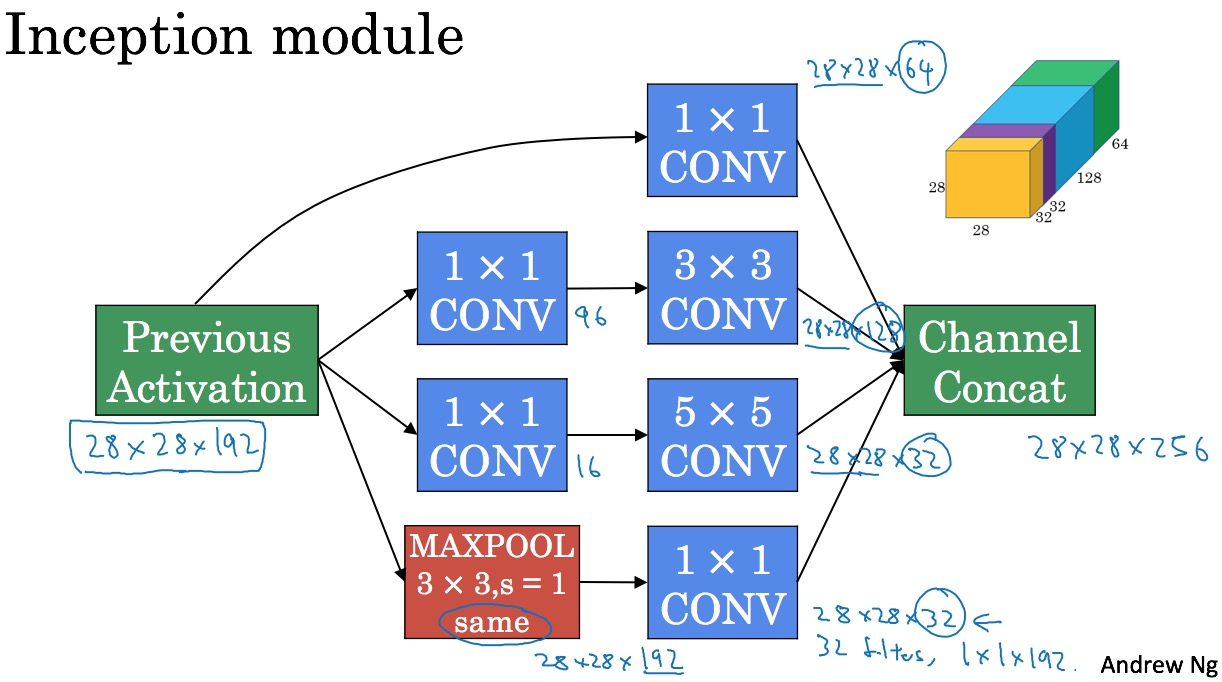
\includegraphics[width=35em]{figures/inception-module}
    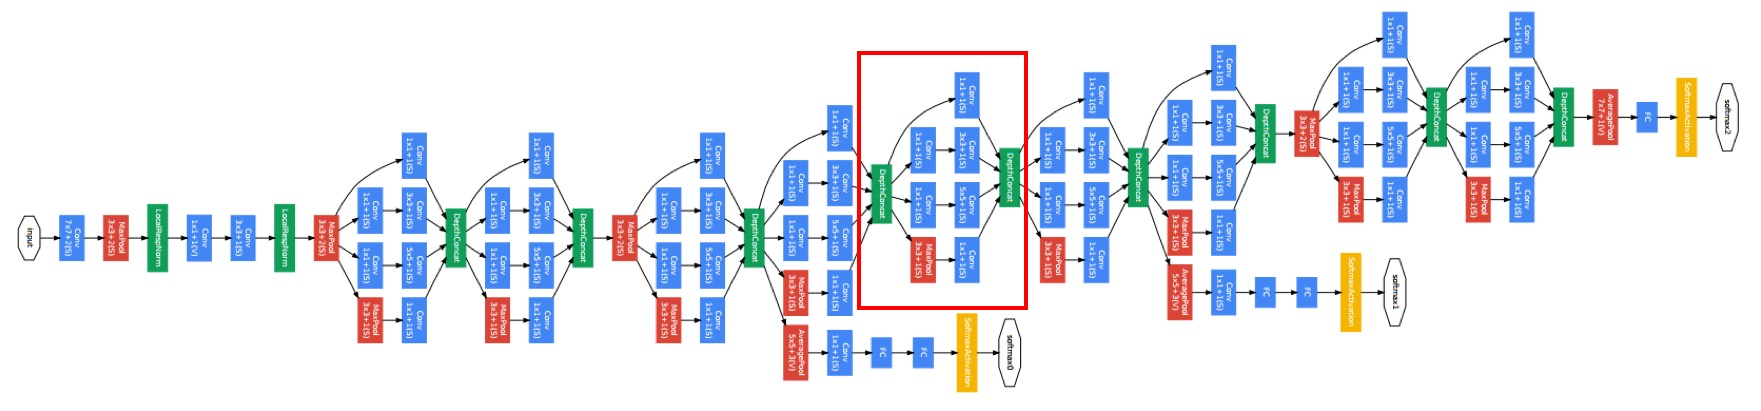
\includegraphics[width=40em]{figures/inception-network}
    \caption{Inception module and Inception Network}
    \label{fig:inception-module-and-inception-network}
\end{figure}

\subsection{Practical advices for using ConvNets}
\subsubsection{Using Open-Source Implementation}
It turns out that a lot of effective neural networks are difficult or finicky to replicate because
a lot of details about tuning the hyperparameters such as learning rate and other things that make
some difference to the performance. Fortunately, a lot of deep learning researchers routinely open
source their work on the internet such as on GitHub.

If you're developing a computer vision application, a very common workflow would be to pick an
architecture that you'd like, and look for an open-source implementation and download it from
GitHub to start building from there. One of the advantages of doing so also is that sometimes these
networks take a long time to train and someone else might have used multiple GPUs in a very largely
dataset to pre-trained some of these networks. And that allows you to do transfer learning using
these networks.

\subsubsection{Transfer Learning}
If you're building a computer vision application, rather training the weights from scratch, from
random initialization, you often make much faster progress if you download weights that someone
else has already trained on a network architecture. And use that as pre-training and transfer that
to a new task that you might be interested in.

The computer vision community has been pretty good at hosting lots of datasets on the Internet. So
if you hear of things like ImageNet or MS COCO types of datasets, there are the names of different
datasets that people have posted online. And a lot of different researchers have trained their
algorithms on.

Sometimes this training takes several weeks, and might take many many GPUs. And the fact that
someone else has done this and gone through the painful high performance search process means that
you can often download open source weights that took someone else many weeks, or months to figure
out. And use that as a very good initialization for your own neural network. And use transfer
learning to sort of transfer knowledge from some of these very large public datasets to your own
problem.

Let's start an example, let's say you're building a cat detector to recognize your own pet cats
Tigger and Misty. So you have a classification problem with three classes, is this picture Tigger,
or is it Misty, or is it neither?

Now, you probably don't have a lot of pictures of Tigger and Misty, so your training set will be
small. You can go online and download some open source implementation of a neural network. And
download not just the code, but also the weights. And there are a lot of networks you can download
that have been trained on. For example, the ImageNet dataset, which has 1,000 different classes.
What you can do is then get rid of the softmax layer, and create your own softmax unit that outputs
Tigger, or Misty, or neither.

\begin{figure}[htb]
    \centering
    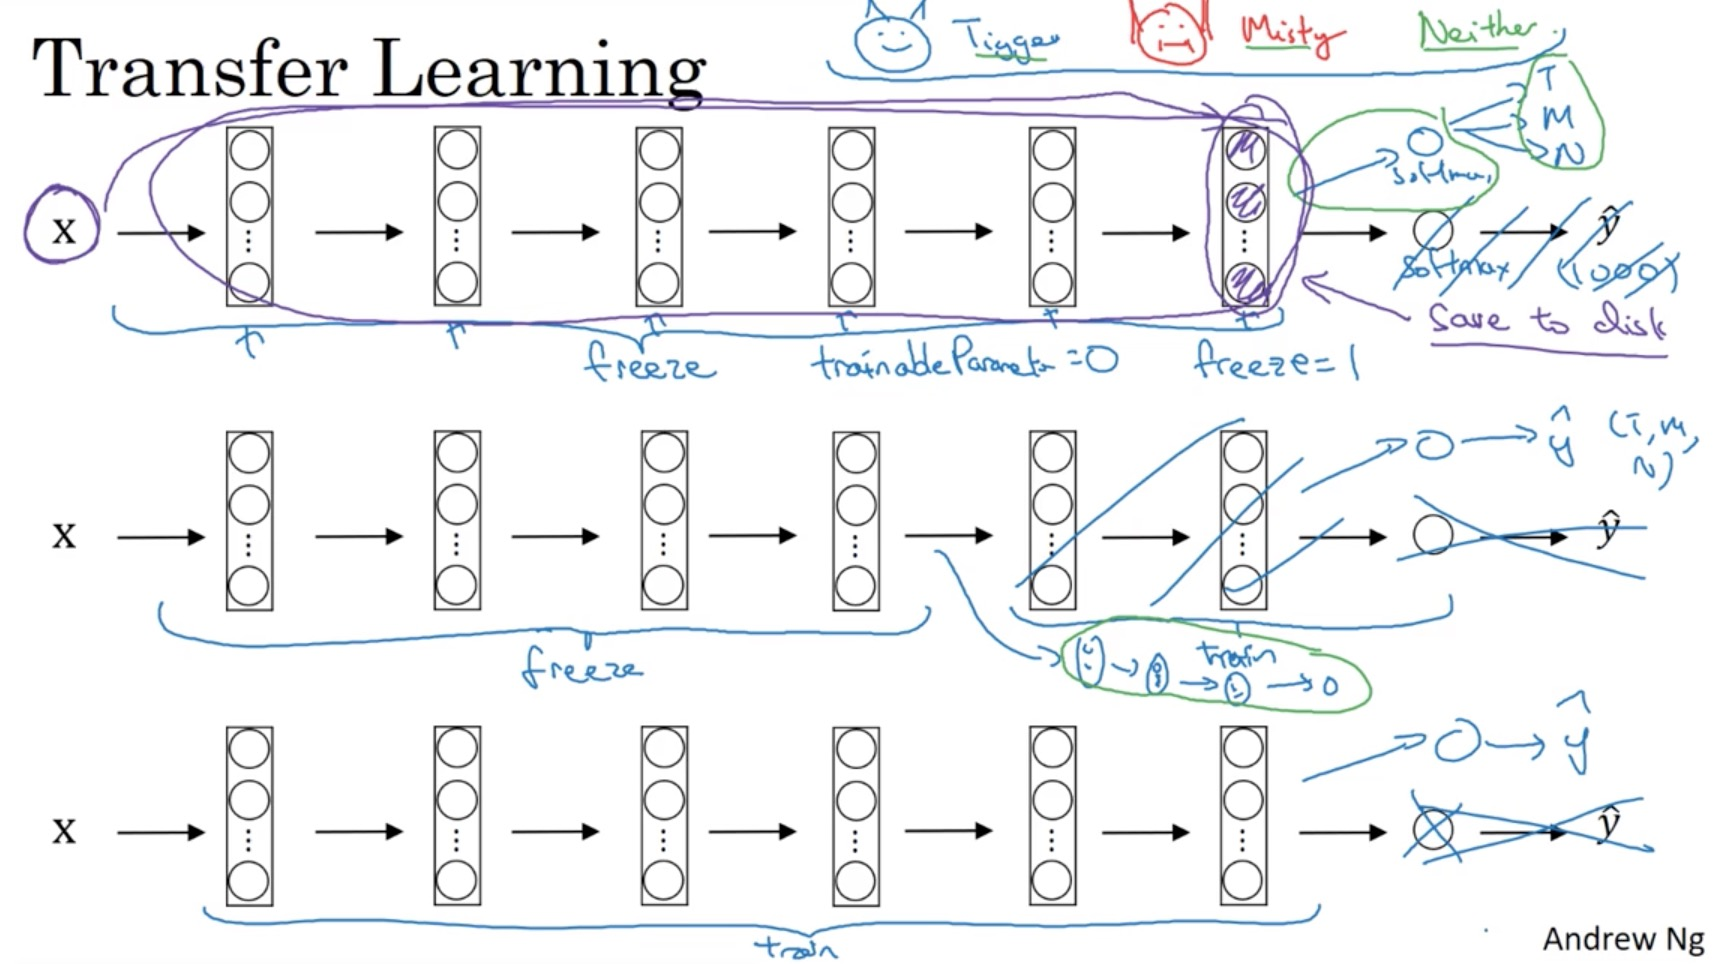
\includegraphics[width=40em]{figures/transfer-learning}
    \caption{Different ways of transfer learning.}
    \label{fig:transfer-learning}
\end{figure}

And in terms of the network, you can freeze the parameters in all the layers before softmax layer
and just train the parameters associated with softmax layer. By using someone else's pre-trained
weights, you're likely to get pretty good performance on this, even with a small dataset.

One other near trick that amy help for some permutations is that, because all of the earlier layers
are frozen, there is some fixed function that doesn't change, because you're not changing it,
you're not training it. That takes as input image $X$ and maps it to some sort of activations in
that layer. So one other trick that could speed up training is if we just pre-compute that layer,
the features or really activations from that layer, and just save them to disk. And what you're
doing is you're using this fixed function, in this part of the neural network, to take as input any
image $X$, and compute some feature vector for it. And then you're training a shallow softmax model
from this feature vector to make a prediction. And so one step that could help your computation is
you just pre-compute that layer's activation for all the examples in your training set, and save
them to disk. And then just train a softmax classifier on top of that. All right, so the advantages
of save to disk or the pre-compute method of save to disk method is that you don't need to recompute
those activations every time you take an epoch, or take a pass through your training set.

If you have a larger labeled dataset, so maybe you just have a ton of pictures of Tigger, Misty,
and as well as, I guess, pictures of neither of them. One thing you could do is then freeze fewer
layers, then train these left layers. And there are a couple of ways to do this, you could take the
last few layers' weights, and just use that as initilization and do gradient descent from there. Or
you could also blow away these last few layers, and just use your own new hidden units, and then
your own final softmax output. So either of these methods could be worth trying.

But maybe one pattern is, if you have more data, the number of layers you freeze could be smaller.
And then the number of layers you train on top could be greater.

\subsubsection{Data Augmentation}
Most computer vision tasks could use more data and so data augmentation is one of the techniques
that is often used to improve the performance of computer vision systems. Computer vision is a
pretty complicated task, and we say we just can't get enough data in this domain.

\begin{itemize}
    \item Common augmentation methods
    \begin{itemize}
        \item Mirroring
        \item Randon Cropping
        \item Rotation
        \item Shearing
        \item Local warping
        \item \ldots
    \end{itemize}
    \item Color shifting (e.g. PCA color augmentation)
\end{itemize}

If your dataset is very large, you can implement distortions (rotation, shearing, \ldots) during
training.

\subsubsection{State of Computer Vision}
If you have lots of data, you can use simpler algorithms, less hand-engineering; while if you have
little data, you need more hand-engineering.

When Andrew Ng looks at machine learning applications, he thinks usually the learning algorithm has
two sources of knowledge. One source knowledge is labeled data, the other is hand-engineering
features/network architectures/other components.

Tips for doing well on benchmarks/winning competitions:
\begin{itemize}
    \item Ensembling
    \begin{itemize}
        \item Train several networks independently and average their outputs
    \end{itemize}
    \item Multi-crop at test time
    \begin{itemize}
        \item Run classifier on multiple versions of test images and average results.
    \end{itemize}
\end{itemize}

Use open source code:
\begin{itemize}
    \item Use architectures of networks published in the literature
    \item Use open source implementations if possible
    \item Use pretrained models and fine-tune on your dataset
\end{itemize}

\section{Object detection}
\subsection{Detection algorithms}
\subsubsection{Object Localization}
Object detection is one of the areas of computer vision that's just exploding and it's working so
much better than just a couple years ago. In order to build up to object detection, you first learn
about object localization. The Figure~\ref{fig:detection-definition} shows the definition of
Detection.

\begin{figure}[htb]
    \centering
    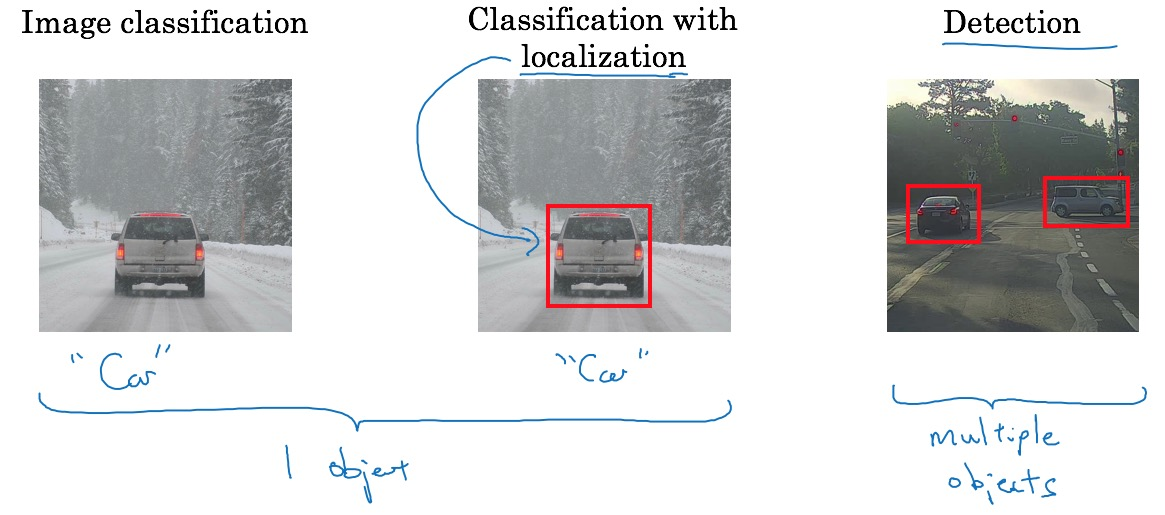
\includegraphics[width=40em]{figures/detection-definition}
    \caption{The definition for Detection}
    \label{fig:detection-definition}
\end{figure}

Classfication algorithm outputs not just a class label but also the four parameters to tell you
where is the bounding box of the object it detected.

There maybe one of the four classses in the image:
\begin{enumerate}
    \item pedestrian
    \item car
    \item motorcycle
    \item background
\end{enumerate}

Target label $\Vector{y}$:
$$ \Vector{y} = \left[\begin{array}{c} p_c \\ b_x \\ b_y \\ b_h \\ b_w \\ c_1 \\ c_2 \\ c_3
\end{array}\right] $$

For example, if the classifier predicts there is a car in the image, then the target label will be
$$ \Vector{y} = \left[\begin{array}{c} 1 \\ b_x \\ b_y \\ b_h \\ b_w \\ 0 \\ 1 \\ 0
\end{array}\right] $$
if the classifier predicts there is no object (just background) in the image, then the target label
will be
$$ \Vector{y} = \left[\begin{array}{c} 0 \\ ? \\ ? \\ ? \\ ? \\ ? \\ ? \\ ? \end{array}\right] $$
where ``$?$'' means ``we don't care''.

If you use squared error, the cost function can be
$$ \Cal{L}(\hat{y}, y) = \left\{\begin{array}{ll} (\hat{y}_1 - y_1)^2 + (\hat{y}_2 - y_2)^2 + \cdots
+ (\hat{y}_8 - y_8)^2 & \text{if } y_1 = 1 \\ (\hat{y}_1 - y_1)^2 & \text{if } y_1 = 0 \end{array}
\right. $$

\subsubsection{Landmark Detection}
In more general cases, you can have a neural network just outputs $x$ and $y$ coordinates of
important points in image, sometimes called the landmarks that you want the neural network to
recognize.

\subsubsection{Object Detection}
\paragraph{Sliding windows detection}
As we can see from Figure~\ref{fig:sliding-window-detection}, by picking a certain window sizes and
then pick the region in the red box as the input of the ConvNet. The ConvNet is a classifiert that
can output the whether the image contains a car (0 or 1). With a fixed stride, then you go
through every region of the image. Last, pick another window size, and repeat over again.

\begin{figure}[htb]
    \centering
    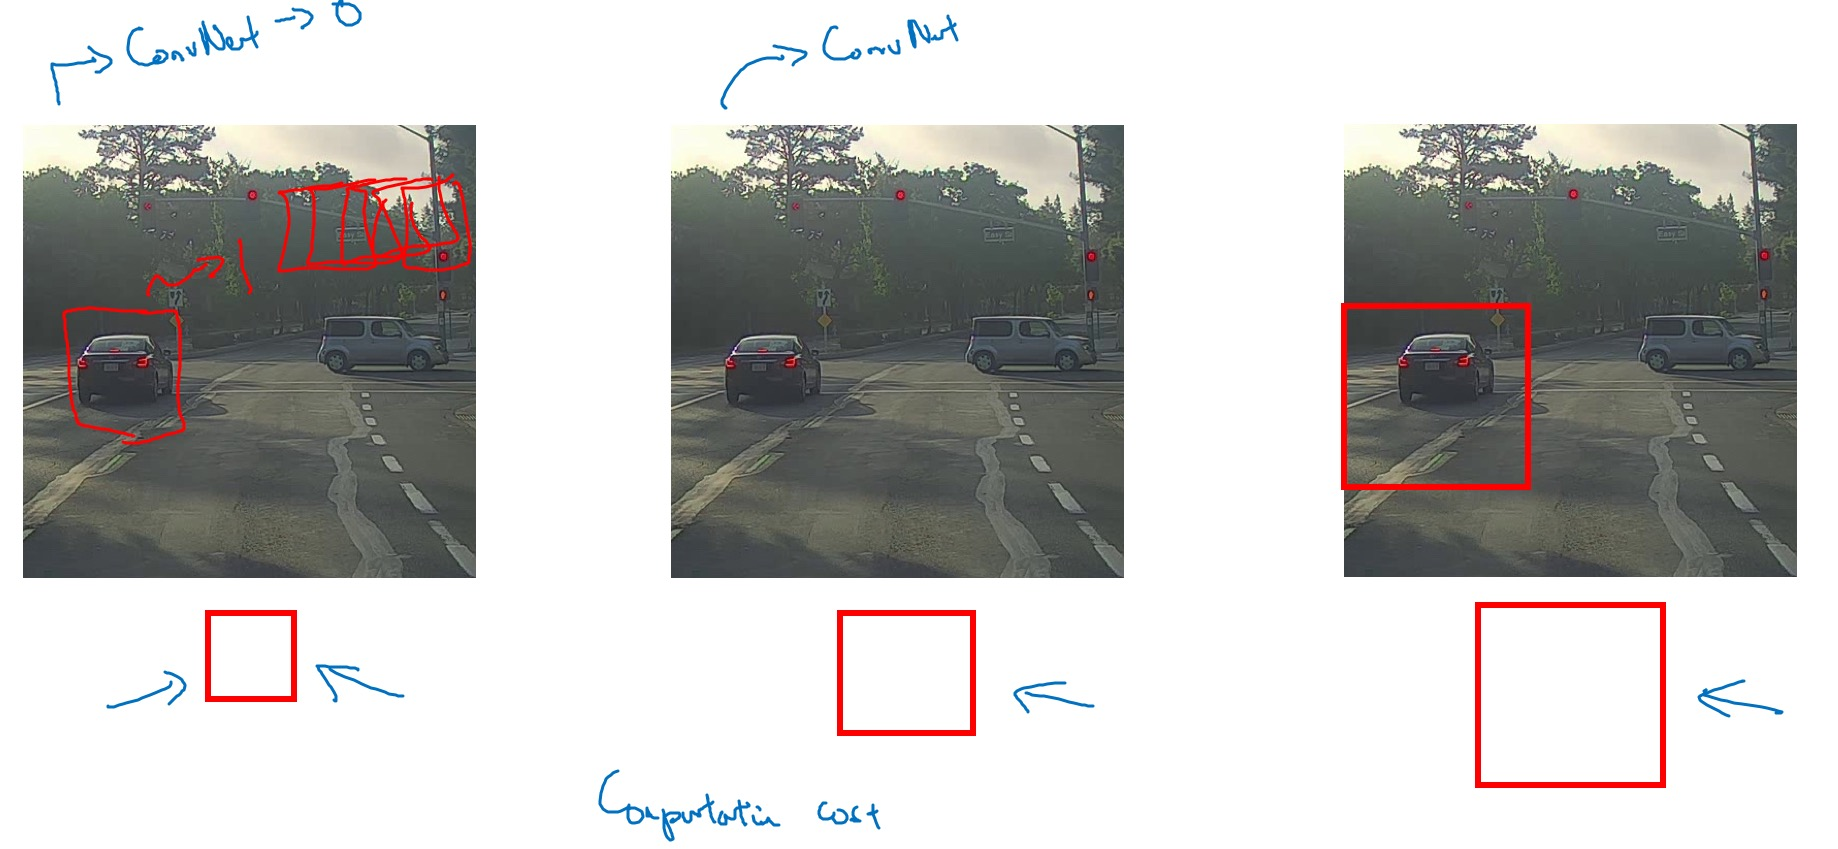
\includegraphics[width=40em]{figures/sliding-window-detection}
    \caption{Sliding window detection}
    \label{fig:sliding-window-detection}
\end{figure}

\subsubsection{Convolutional Implementation of Sliding Windows}
\paragraph{Turning FC layers into convolutional layers}
Figure~\ref{fig:turning-fc-layer-into-conv-layers} shows how to turn FC layer into 1 $\times$ 1
CONV layers.

\begin{figure}[htb]
    \centering
    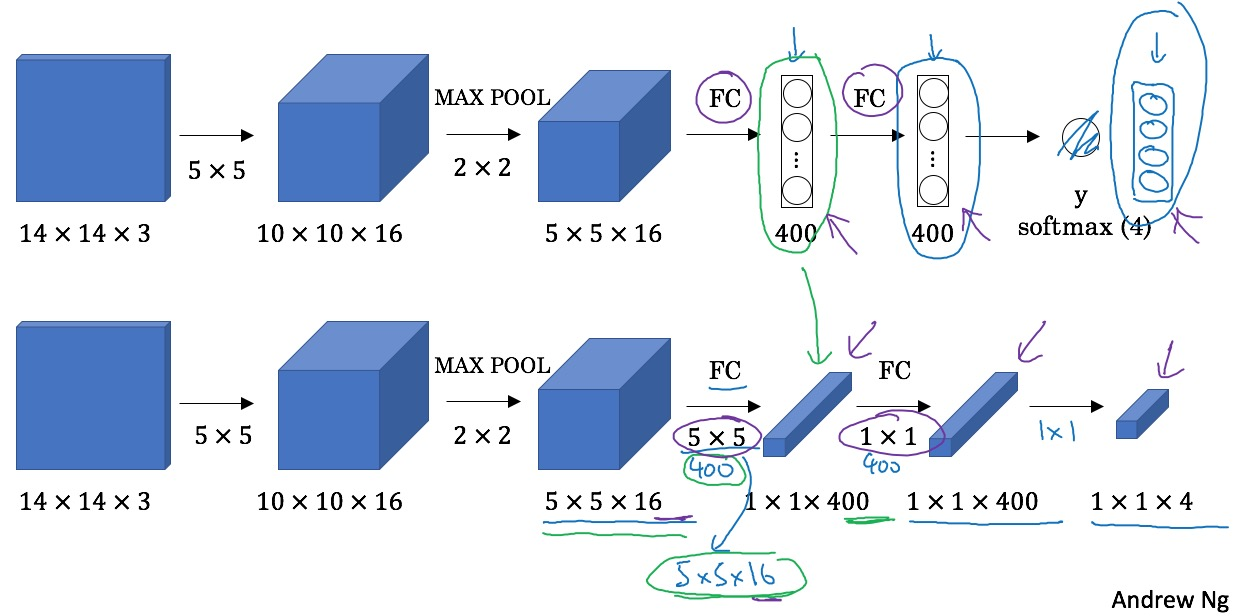
\includegraphics[width=40em]{figures/turning-fc-layer-into-conv-layers}
    \caption{Turning FC layer into CONV layers}
    \label{fig:turning-fc-layer-into-conv-layers}
\end{figure}

\paragraph{Convolutional implementation of sliding windows}
Like Figure~\ref{fig:conv-implementation-of-sliding-windows} shows, the ConvNet inputs 14 $\times$
14 $\times$ 3 images and your test set image is 16 $\times$ 16 $\times$ 3 so now added that yellow
stide to the border of the image. So in the original sliding windows algorithm, you might want to
input the blue region into a ConvNet and run that once to generate a classification 0 or 1 and
then slide it down a bit.

Originally, to run sliding windows on this 16 $\times$ 16 $\times$ 3 image, you run the 14 $\times$
14 $\times$ 3 ConvNet four times in order to get 4 labels. But it turns out a lot of this
computation done by these 4 ConvNets is highly duplicated. So what the convolutional implementation
of sliding windows does is it allows these 4 forward passes of the ConvNets to share a lot of
computation.

\begin{figure}[htb]
    \centering
    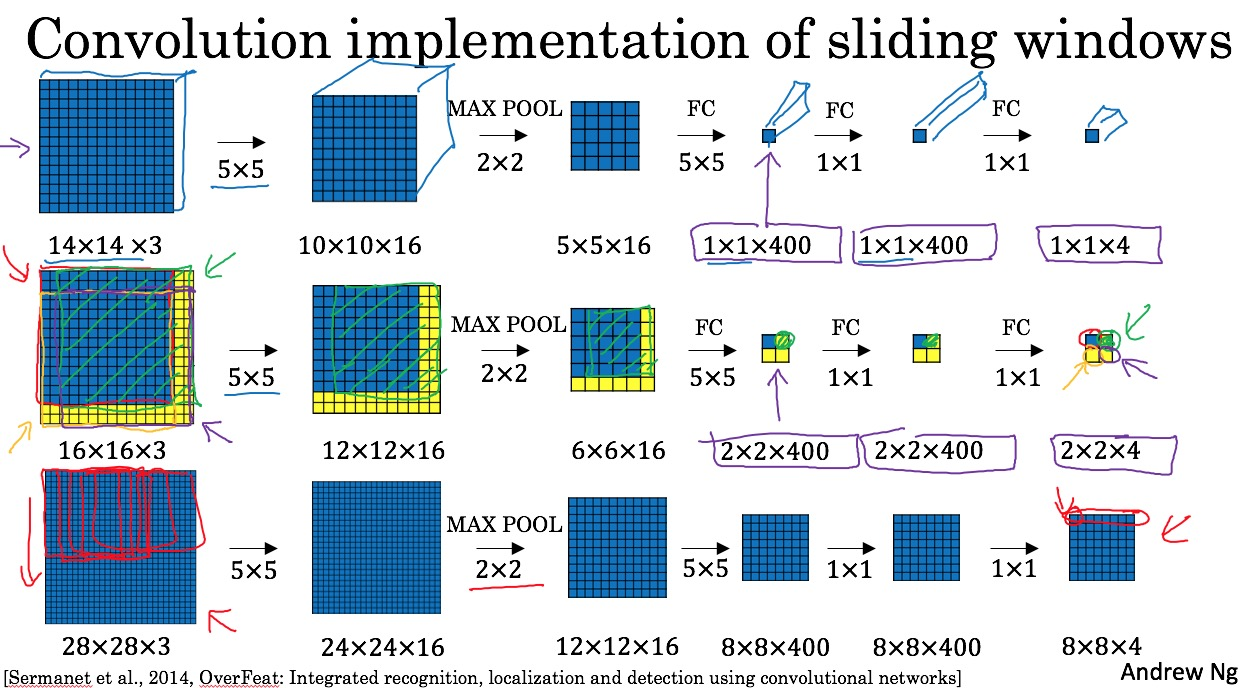
\includegraphics[width=40em]{figures/conv-implementation-of-sliding-windows}
    \caption{Convolution implementation of sliding windows}
    \label{fig:conv-implementation-of-sliding-windows}
\end{figure}

\subsubsection{Bounding Box Predictions}
Using a convolutional implementation of sliding windows is more computationally efficient but the
it's still have a problem of not quite outputting the most accurate bouding boxes.

\paragraph{YOLO algorithm}
``YOLO'' means ``You Only Look Once''.

Let's say you have an input image that is 100 $\times$ 100, you're going to place down a grid on
this image and for the purposes of illustration, we use 3 $\times$ 3 grid.

The basic idea is that you are going to take the image classification and localization algorithm
and apply it to each of the nine grid cells of this image. So the more concrete here's how you
define the labels you use for training.

For each grid cell:
$$ \Vector{y} = \left[\begin{array}{c} p_c \\ b_x \\ b_y \\ b_h \\ b_w \\ c_1 \\ c_2 \\ c_3
\end{array}\right] $$

To give a bit more detail, if the image contains two objects, what the YOLO algorithm does is it
takes the midpoint of each of the two objects and it assigns the object to the grid cell containing
the midpoint. And so even though some grid cells have some parts of the cars will pretend that it
has no interesting object.

How to specify the bounding box? In the YOLO algorithm, relative to one grid cell, we take the
convention that the upper-left point is $(0, 0)$ and the lower-right point is $(1, 1)$, refers to
Figure~\ref{fig:bounding-boxes}. To specify the position of the midpoint of interesting object. The
$b_x$, $b_y$, $b_h$, $b_w$ are specified relative to the grid cell. So $b_x$ and $b_y$ are must
between 0 and 1, but $b_h$ and $b_w$ could be larger than 1.

\begin{figure}[htb]
    \centering
    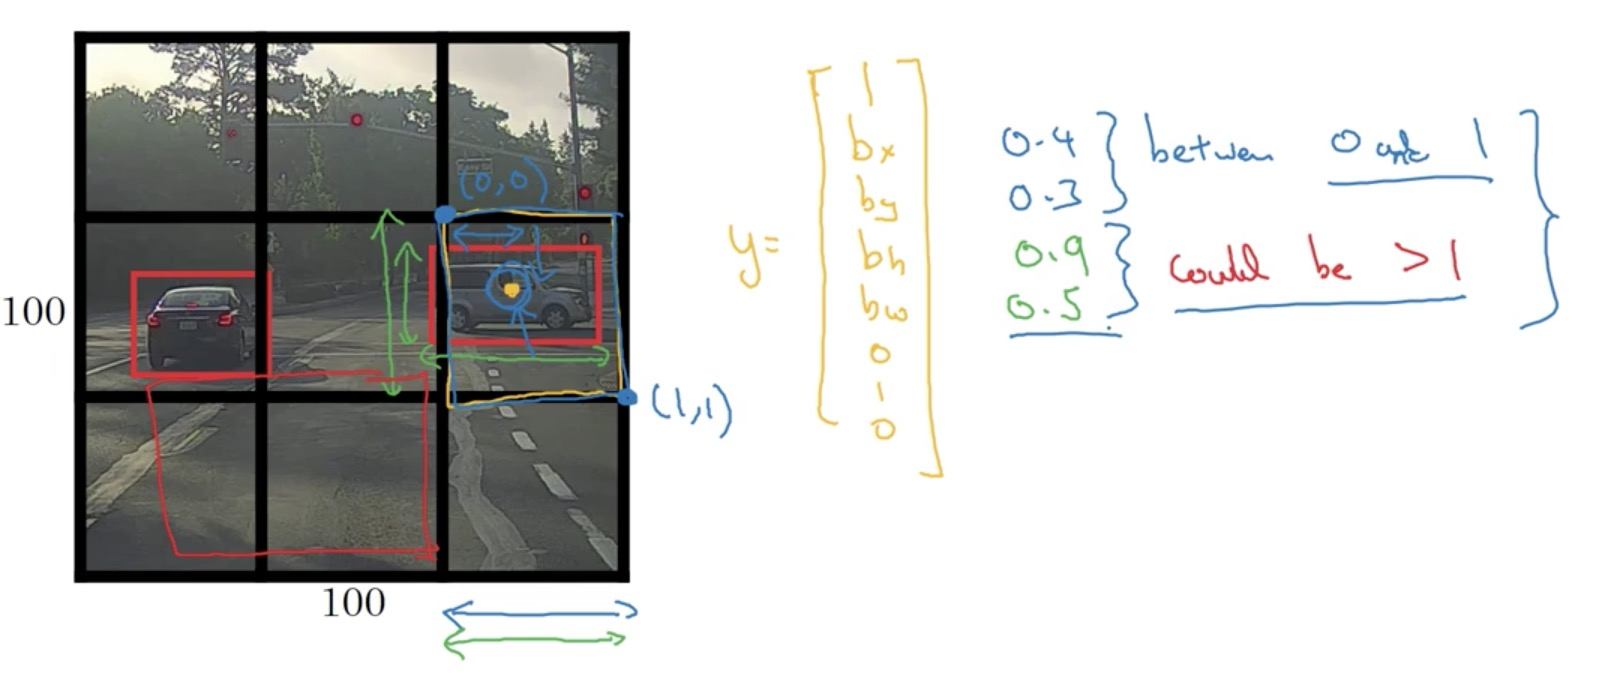
\includegraphics[width=40em]{figures/bounding-boxes}
    \caption{Specify the bounding boxes}
    \label{fig:bounding-boxes}
\end{figure}

\subsubsection{Intersection over Union}
$IoU$, which means Intersection over Union, Figure~\ref{fig:IoU}. More generally, $IoU$ is a
measure of the overlap between two bounding boxes.

\begin{figure}[htb]
    \centering
    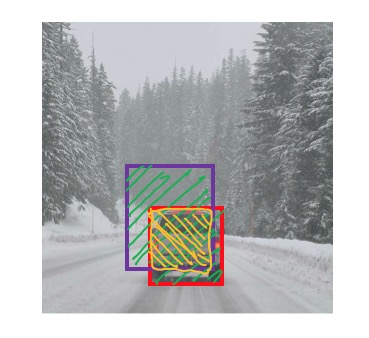
\includegraphics[width=25em]{figures/IoU}
    \caption{IoU}
    \label{fig:IoU}
\end{figure}

$$ IoU = \frac{\text{size of intersection}}{\text{size of union}} $$

Maybe we think the bounding box is correct only if $IoU \geq 0.5$.

\subsubsection{Non-max Suppression}
One of the problems of object detection as you've learned about so far is that your algorithm may
find multiple detections of the same object so rather than detecting an object just once, it might
detect it multiple times. Non-max suppression is a way for you to make sure that your algorithm
detects each object only once.

Like Figure~\ref{fig:non-max-surppression-example} shows, we will run image and localization
algorithm on every grid cell on 361 grid cells. It's possible that many of them will raise their
hand and say my $p_c$ chance of thinking I've an object in it. So when you run your algorithm, you
might end up with multiple detections of each ojbect. What non-max suppression does is it clean up
these detections and end upo with just one detection per car rather than multiple detections per
car.

\begin{figure}[htb]
    \centering
    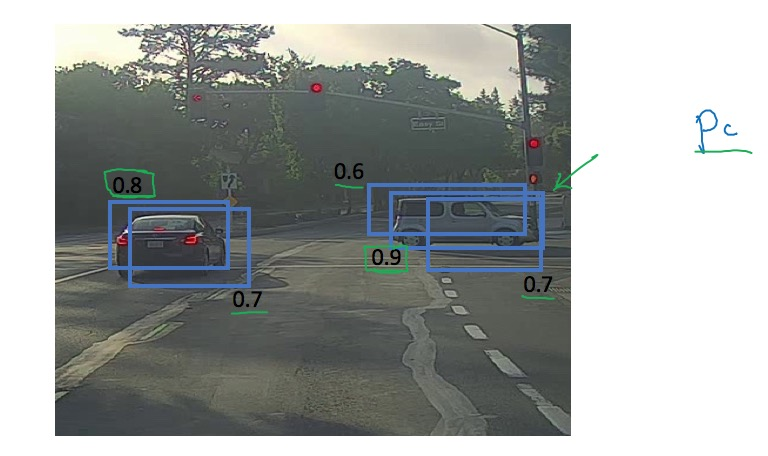
\includegraphics[width=25em]{figures/non-max-surppression-example}
    \caption{Non-max surppression example}
    \label{fig:non-max-surppression-example}
\end{figure}

Concretely what it does is it first looks at the probabilities associated with each of these
detection. It first takes the largest one which in this case is 0.9 and says that's my most
confident detection so let's highlight that I'm just say I found a car there. Having done that the
non-max suppression part then looks at all of remaining rectangles and all the ones with a high
overlap ($IoU$) with this one you've just output will get suppressed. Next you then go through the
remaining and find the one with the highest probability ($p_c$) and repeat the above steps.

\begin{enumerate}
    \item On 19 $\times$ 19 grid you're going to run and get a 19 $\times$ 19 $\times$ 8 output
    volume. Although for this example, to simplify it to say that you're only doing car detection
    so we get rid of the $c_1$, $c_2$ and $c_3$. Then each output prediction we get is:
    $\displaystyle \left[\begin{array}{c} p_c \\ b_x \\ b_y \\ b_h \\ b_w \end{array}\right]$
    \item Discard all boxes with $p_c \leq 0.6$
    \item While there are any remaining boxes:
    \begin{itemize}
        \item Pick the box with the largest $p_c$, output that as a prediction.
        \item Discard any remaining box with $IoU \geq 0.5$ with the box output in the previous
        step
    \end{itemize}
\end{enumerate}

\subsubsection{Anchor Boxes}
One of the problems with object detection as you've seen it so far is that each of the grid cells
can detect only one object whatever grid cell wants to detect multiple objects. What if grid cells
want to detect multiple objects? We can use anchor boxes.

See the example shows in Figure~\ref{fig:anchor-boxes-example}. In this example, notice that the
midpoint of the pedestrian and the midpoint of the car are in almost the same place and both of
them fall into the same grid cell. But it won't be able to output two detections so you have to pick
one of the two detections to output.

With the idea of anchor boxes, what you're going to do is predefined two different shapes called
anchor boxes or anchor boxes shapes. And what you're going to do is now be able to associate two
predictions with the two anchor boxes. Define
$$ \Vector{y} = \left[\begin{array}{c} p_c^{(1)} \\ b_x^{(1)} \\ b_y^{(1)} \\ b_h^{(1)} \\ b_w^{(1)}
\\ c_1^{(1)} \\ c_2^{(1)} \\ c_3^{(1)} \\ p_c^{(2)} \\ b_x^{(2)} \\ b_y^{(2)} \\ \vdots \\ c_3^{(2)}
\end{array}\right]
\begin{array}{llll} \left.\begin{array}{c} \\ \\ \\ \\ \\ \\ \\ \\ \\ \end{array}\right\}
\begin{array}{c}\text{anchor box 1}\end{array} \\
\left.\begin{array}{c} \\ \\ \\ \\ \\ \\ \end{array}\right\}
\begin{array}{c}\text{anchor box 2}\end{array} \end{array} $$

\begin{figure}[htb]
    \centering
    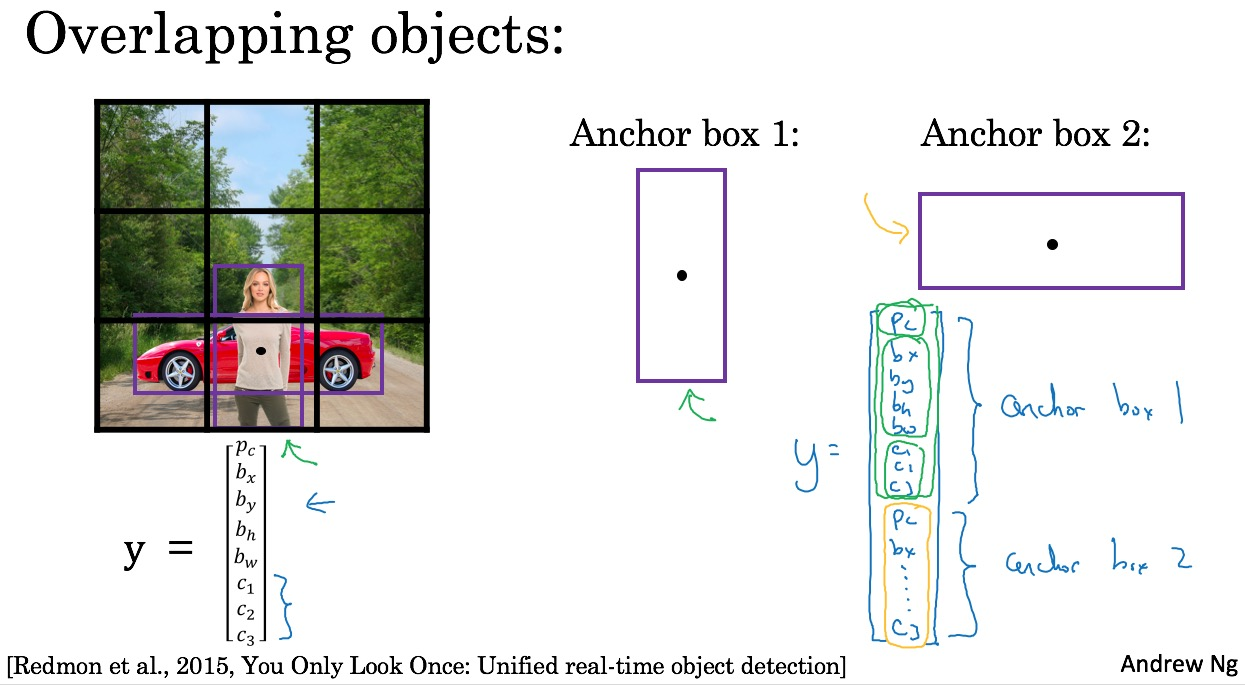
\includegraphics[width=40em]{figures/anchor-boxes-example}
    \caption{Anchor boxes example}
    \label{fig:anchor-boxes-example}
\end{figure}

Previously: Each object in training image is assigned to grid cell that contains that object's
midpoint. Output $\Vector{y}$: 3 $\times$ 3 $\times$ 8.

With two anchor boxes: Each object in training image is assigned to grid cell that contains object's
midpoint and anchor box for the grid cell with highest $IoU$. Output $\Vector{y}$: 3 $\times$ 3
$\times$ 16.

\subsubsection{YOLO algorithm}
Suppose you are trying to train an algorithm to detect three objects, pedestrians, cars and
motorcycle. If you're using two anchor boxes, your output $\Vector{y}$ will be 3 $\times$ 3
$\times$ 2 $\times$ 8.

\begin{enumerate}
    \item Training
    \item Making predictions
    \item Outputting the non-max suppressed outputs
    \begin{itemize}
        \item For each grid call, get 2 predicted bounding boxes.
        \item Get rid of low probability predictions.
        \item For each class (pedestrain, car, motorcycle), use non-max suppression to generate
        final predictions.
    \end{itemize}
\end{enumerate}

\subsubsection{Region Proposals}
Region proposal: R-CNN.
\begin{enumerate}
    \item Use segmentation algorithms to find blobs with bounding boxes.
    \item Run classifier on the blobs.
\end{enumerate}

R-CNN: Propose regions. Classify proposed regions one at a time. Output label and bounding boxes.

Fast R-CNN: Propose regions. Use convolution implementation of sliding windows to classify all the
proposed regions.

Faster R-CNN: Use convolution network to propose regions.


\section{Special applications: Face recognition \& Neural style transfer}
\subsection{Face Recognition}
\subsubsection{What is face recognition?}
Face verification vs. face recognition

Verification
\begin{itemize}
    \item Input image, name/ID
    \item Output whether the input image is that of the claimed person
\end{itemize}

Recognition
\begin{itemize}
    \item Has a database of $K$ persons
    \item Get an input image
    \item Output ID if the image is any of the $K$ persons (or ``not recognized'')
\end{itemize}

\subsubsection{One Shot Learning}
One of the challenges of face recognition is that you need to solve the one-shot learning problem.
What that means is that for most face recognition applications you need together recognize a person
given just one single image or given just one example of that person's face.

Softmax function doesn't work well on this problem, because if you have such a small training set,
it is not enough to train a robust neural network for this task. And whatever new person joins your
team, so now you have to retrain the ConvNets every time.

\paragraph{Learning a ``similarity'' function}
$$ d(img1, img2) = \text{degree of difference between images} $$

If $d(img1, img2) \leq \tau$, predict ``same''; if $d(img1, img2) > \tau$, predict ``different''.

\subsubsection{Siamese network}
Like Figure~\ref{fig:siamese-network} shows, say we have two images $x^{(1)}$ and $x^{(2)}$, and
we want to judge if they are the same person. What we can do is input the two images to Simamese
network independently, and get their encoding $f(x^{(1)})$ and $f(x^{(2)})$. Then we use $L_2$ Norm
as the similarity function
$$ d(x^{(1)}, x^{(2)}) = ||f(x^{(1)}) - f(x^{(2)})||_2^2 $$

\begin{figure}[htb]
    \centering
    \includegraphics[width=40em]{figures/siamese-network}
    \caption{Siamese network}
    \label{fig:siamese-network}
\end{figure}

Parameters of NN define an encoding $f(x^{(i)})$. Learn parameters so that if $x^{(i)}$, $x^{(j)}$
are the same person, $||f(x^{(i)}) - f(x^{(j)})||_2^2$ is small; if $x^{(i)}$, $x^{(j)}$ are
different persons, $||f(x^{(i)}) - f(x^{(j)})||_2^2$ is large.

\subsubsection{Triplet Loss}
One way to learn the parameters of the neural network so that it gives you a good encoding for your
images of faces is to define and apply gradient descent on the triplet loss function.

\paragraph{Learning Objective}
Given an Anchor image $A$, for each Positive image $P$ and Negative image $N$, we want
$$ \underbrace{||f(A)-f(P)||^2}_{d(A, P)} \leq \underbrace{||f(A)-f(N)||^2}_{d(A, N)} $$

$$ ||f(A)-f(P)||^2 - ||f(A)-f(N)||^2 \leq 0 $$

To prevent $f(img) = \Vector{0}$
$$ ||f(A)-f(P)||^2 - ||f(A)-f(N)||^2 + \alpha \leq 0 $$
where $\alpha$ is a hyperparameter, also called ``margin'', it can push the anchor positive pair
and the anchor negative pair further away from each other.

\paragraph{Loss function}
Given 3 images, $A$, $P$, $N$, on a single triplet:
$$ \Cal{L}(A, P, N) = \text{max}(||f(A)-f(P)||^2 - ||f(A)-f(N)||^2 + \alpha, 0) $$

Overall cost function:
$$ J = \sum_{i=1}^m \Cal{L}(A^{(i)}, P^{(i)}, N^{(i)}) $$

\paragraph{Choosing the triplets $A$, $P$, $N$}
During training, if $A$, $P$, $N$ are chosen randomly, $d(A, P) + \alpha \leq d(A, N)$ is easily
satisfied, so the network won't learn much in this way.

Choose triplets that are ``hard'' to train on:
$$ d(A, P) + \alpha \leq d(A, N) $$
$$ d(A, P) \approx d(A, N) $$

\subsubsection{Face verification and binary classification}
The triplet loss is one good way to learn the parameters of a ConvNet for face recognition. Face
recognition can also be posed as a straight binary classification problem.

Another way to train a neural network is to take the pair of neural networks to take Siamese
network and have them both compute the 128 dimensional embeddings. And then have these be input to
a logistic regression unit to make a prediction, where the target output will be 1 if both of these
are same persons and 0 if both of these are of different persons. So like
Figure~\ref{fig:face-verification-and-binary-classification} shows, this is a way to treat face
recognition just as a binary classificaion problem.

\begin{figure}[htb]
    \centering
    \includegraphics[width=40em]{figures/face-verification-and-binary-classification}
    \caption{Learning the similarity function}
    \label{fig:face-verification-and-binary-classification}
\end{figure}

$$ \hat{y} = \sigma(\sum_{k=1}^{128} w_i ||f(x^{(i)})_k - f(x^{(j)})_k|| + b) $$
or
$$ \hat{y} = \sigma(\sum_{k=1}^{128} w_i \frac{(f(x^{(i)})_k - f(x^{(j)})_k)^2}{f(x^{(i)})_k
+ f(x^{(j)})_k} + b) $$
where $\displaystyle \frac{(f(x^{(i)})_k - f(x^{(j)})_k)^2}{f(x^{(i)})_k + f(x^{(j)})_k}$ is
sometimes called $\chi^2$ similarity.

\paragraph{Face verification supervised learning}
To treat face verification as supervised learning, you create a training set of just pairs of
images now, instead of triplets. And pairs of images where the target label is 1 when these are
a pair of pictures of the same person and where the target label is 0 when these are pictures of
different persons. So you use pairs of images to train the Siamese network using backpropagation.

\subsection{Neural Style Transfer}
\subsubsection{What is neural style transfer?}
One of the most fun and exciting applications of ConvNets recently has been neural style transfer.

Figure~\ref{fig:neural-style-transfer-examples} shows two examples of neural style transfer. We use
$C$ to denote the Content image, $S$ to denote the Style image, and $G$ to denote the generated
image.

\begin{figure}[htb]
    \centering
    \includegraphics[width=40em]{figures/neural-style-transfer-examples}
    \caption{Neural style transfer examples}
    \label{fig:neural-style-transfer-examples}
\end{figure}

\subsubsection{What are deep ConvNets learning?}
\paragraph{Visualizing what a deep network is learning}
Pick a unit layer 1. Find the nine image patches that maximize the unit's activation. Then repeat
for other units.

Repeat the procedure and you can visualize more deep layers.

\subsubsection{Cost function}
$$ J(G) = \alpha J_{\text{content}}(C, G) + \beta J_{\text{style}}(S, G) $$

$J_{\text{content}}$ measures how similar the contents of the generated image is to the content of
Content image. $J_{style}$ measures how similar to the style of the generated image is to the style
of the Style image.

\paragraph{Find the generated image $G$}
\begin{enumerate}
    \item Initiate $G$ randomly \\
    e.g. $G$ 100 $\times$ 100 $\times$ 3
    \item Use gradient descent to minimize $J(G)$
    $$ G := G - \frac{\partial}{\partial G} J(G) $$
\end{enumerate}

\subsubsection{Content Cost Function}
\begin{itemize}
    \item Say you use hidden layer $l$ to compute content cost.
    \begin{itemize}
        \item If $l$ is a very small number, if you used in there 1, then it would really force your generated
        image and the pixel values very similar to your Content image; whereas if you use a very deep
        layer, then it's just asking well if there's a dog in your content image then make sure there's a
        dog somewhere in the generated image. So in practice, the layer $l$ is chosen somewhere in between
        is neither too shallow nor too deep in the neural network.
    \end{itemize}
    \item Use pre-trained ConvNet. (E.g., VGG network)
    \item Let $a^{[l](C)}$ and $a^{[l](G)}$ be the activation of layer $l$ on the images
    \item If $a^{[l](C)}$ and $a^{[l](G)}$ are similar, both images have similar content
\end{itemize}

$$ J_{\text{content}}(C, G) = \frac{1}{2} ||a^{[l](C) - a^{[l][G]}}||^2 $$

\subsubsection{Style Cost Function}
\begin{itemize}
    \item Say you are using layer $l$'s activation to measure ``style''.
    \item Define style as \emph{correlation} between activations across channels.
    \begin{itemize}
        \item The correlation tells you which of these high level texture components tend to occur
        or not occur together in part of the image.
    \end{itemize}
    \item Compute Style matrix (Gram matrix)
    \begin{itemize}
        \item Let $a_{i,j,k}^{[l]} = \text{activation at } (i, j, k).$ \quad $G^{[l]}$ is $n_C^{[l]}
        \times n_C^{[l]}$
        \item Define and compute the Style matrix
        $$ G_{kk'}^{[l](S)} = \sum_{i=1}^{n_H^{[l]}} \sum_{j=1}^{n_W^{[l]}} a_{ijk}^{[l](S)}
        a_{ijk'}^{[l](S)} $$
        $$ G_{kk'}^{[l](G)} = \sum_{i=1}^{n_H^{[l]}} \sum_{j=1}^{n_W^{[l]}} a_{ijk}^{[l](G)}
        a_{ijk'}^{[l](G)} $$
    \end{itemize}
\end{itemize}

$$ J_{\text{style}}^{[l]}(S, G) = \frac{1}{(2 n_H^{[l]} n_W^{[l]} n_C^{[l]})^2}
|| G^{[l](S)} - G^{[l](G)} ||_F^2 = \frac{1}{(2 n_H^{[l]} n_W^{[l]} n_C^{[l]})^2} \sum_k \sum_{k'}
(G_{kk'}^{[l](S)} - G_{kk'}^{[l](G)}) $$

It turns out that you get more visually better result if you use the sum of cost functions from
multiple different layers.

The overall style cost function
$$ J_{\text{style}}(S, G) = \sum_l \lambda^{[l]} J_{\text{style}}^{[l]}(S, G) $$

\subsubsection{1D and 3D Generalizations}
Like Figure~\ref{fig:conv-nets-on-1d-data} and Figure~\ref{fig:conv-nets-on-3d-data} shows,
ConvNets can also be used on 1D and 3D data.

\begin{figure}[htb]
    \centering
    \includegraphics[width=40em]{figures/conv-nets-on-1d-data}
    \caption{Convolution in 2D and 1D}
    \label{fig:conv-nets-on-1d-data}
\end{figure}

\begin{figure}[htb]
    \centering
    \includegraphics[width=40em]{figures/conv-nets-on-3d-data}
    \caption{3D convolution}
    \label{fig:conv-nets-on-3d-data}
\end{figure}

For a long upon 1D data applications you actually use a Recurrent Neural Network, but some people
also try using ConvNets in these problems.
















\end{document}
